\documentclass[10pt, a4paper,twoside]{scrartcl}
\usepackage{amsmath}
\usepackage{amssymb}
\usepackage{graphicx}
\usepackage{subcaption}
\usepackage{float}
\usepackage[top=2cm,bottom=3cm,outer=2cm,inner=3cm]{geometry}\usepackage[utf8]{inputenc}
\usepackage{hyperref}
\usepackage[multiple]{footmisc}
\usepackage{parskip}
\usepackage{wrapfig}
\usepackage{xfrac}
\usepackage{xcolor}
\usepackage{tikz}
\usetikzlibrary{arrows}
\usetikzlibrary{arrows.meta}
\usepackage{longtable}
\usepackage{pdfpages}
\usepackage[tikz]{bclogo}
\usepackage{eurosym}
\usepackage{listings}

\hypersetup{
    colorlinks=true,
    linkcolor=blue,
    filecolor=magenta,      
    urlcolor=cyan
}

\restylefloat{table}

\newcommand{\warn}[1]{\textbf{#1}}
\newcommand{\con}[1]{\texttt{#1}}
\newcommand{\dis}[1]{\textbf{\texttt{#1}}}

\newenvironment{remember}{\begin{bclogo}[couleur=blue!30,arrondi=.1,logo=\bccrayon,ombre=true]{Remember}}{\end{bclogo}}   
\newenvironment{remark}{\begin{bclogo}[couleur=blue!30,arrondi=.1,logo=\bcinfo,ombre=true]{Remark}}{\end{bclogo}}   
\newenvironment{warning}{\begin{bclogo}[couleur=red!30,arrondi=.1,logo=\bcattention,ombre=true]{Warning}}{\end{bclogo}}   


\title{QRP CW Transceiver Manual}
\subtitle{Board rev. 2, Firmware rev. 2.0}
\author{Hannes Matuschek -- DM3MAT\\\texttt{<dm3mat [at] darc [dot] de>}\\\texttt{https://dm3mat.darc.de/cw2019}}
\date{\today}

\begin{document}
\maketitle

\begin{abstract}
This document describes the assembly, alignment and usage of the second revision of my small, portable CW TRX. If you cannot find any \emph{rev 2} markings on your boards, this is the wrong document!

The main difference to the first revision is the mixer. Instead of a \texttt{74HC4053}, which has some significant damping on higher frequencies, the second revision relies on the famous \texttt{FST3253} switch. This allows for using the TRX well into the 10m band. Additionally, the board layout has been changed to allow for board-to-board interconnects and proper connectors to ease the assembly of the final TRX. To this end there are only two boards (instead of three) with a $10\times 8\,cm$ footprint that can be squeezed into a $10 \times 10\times 5\,cm$ Fischer-chassis (\texttt{KOH-2100} + \texttt{KOH-4100} + \texttt{DPL 2-4}).  Using this chassis, the receiver will weight about $580\,g$ (without batteries \& key).
\end{abstract}
\thispagestyle{empty}
\vfill
\begin{center}
 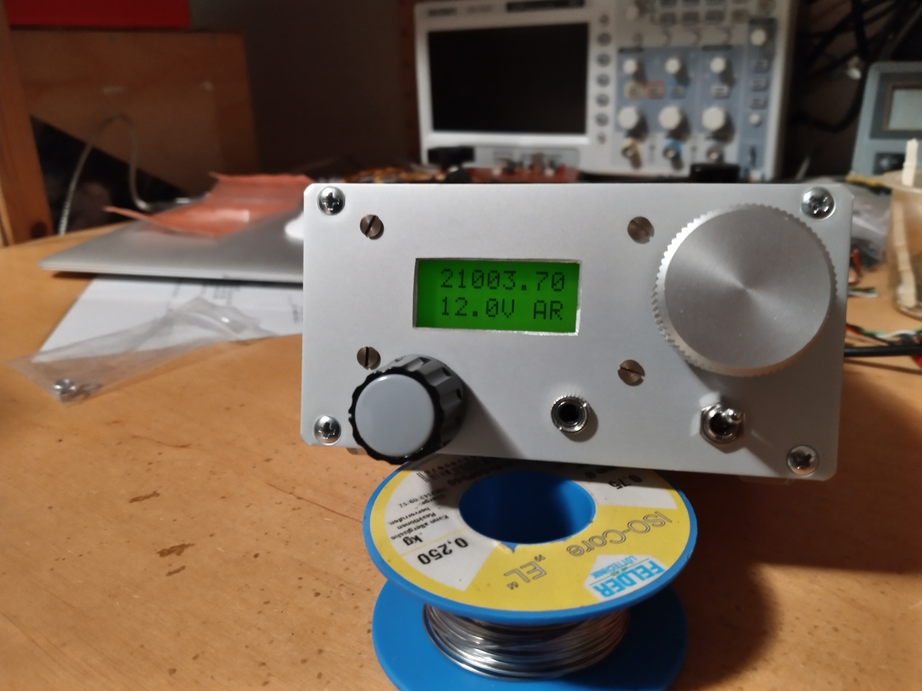
\includegraphics[width=0.7\linewidth]{fig/complete_small.png}
\end{center}



\cleardoublepage
\tableofcontents
\thispagestyle{empty}

\cleardoublepage
\section{Receiver \& Controller Board} \label{sec:rx}
 The receiver and controller board houses the majority of the TRX circuitry. The receiver is a direct conversion receiver using the \texttt{FST3253} CMOS switch as a sample-hold mixer (in conjunction with \texttt{C4-C7}). The latter takes two VFO input signals with $90^\circ$ phase difference and produces four mixing products with $0^\circ$, $90^\circ$, $180^\circ$ and $270^\circ$ phase shifts. These signal pairs ($0^\circ$ + $180^\circ$) and ($90^\circ$ + $270^\circ$) are fed into two independent difference-amplifiers (\texttt{U6A}, \texttt{U6B}) producing two $90^\circ$ phase-shifted audio signals (for USB, $-90^\circ$ for LSB). The following phase-shift-network \texttt{U7} \& \texttt{U8} then shifts back the audio phase by $-90^\circ$ at $700\,Hz$. Finally the resulting signals are added at \texttt{RV3}. Here the USB signals will interfere constructively while the LSB signals will cancel out. This phasing method allows for an unwanted side-band suppression in a direct conversion receiver. The next stages (\texttt{U3} \& \texttt{U5}) will filter and amplify audio signals near $700\,Hz$, which are then fed into the audio PA \texttt{U4}. 
 
 The controller and VFO section of the board consists of a \texttt{ATMega 328P} MCU controlling the \texttt{SI5351} PLL oscillator. The \texttt{CLK2} signal of the PLL drives the two flip-flops \texttt{U9}, which divide the \texttt{CLK2} frequency by four and produce a proper $90^\circ$ phase-shifted signal for the mixer.
 
\subsection{Controller Assembly}
 In a first step, the controller section of the receiver board is assembled. Install \texttt{C2}, \texttt{C26}, \texttt{J7} connector, \texttt{L2}, \texttt{C40}, \texttt{C41}, \texttt{C42}, \texttt{U10}, \texttt{J10}, \texttt{C14}, \texttt{J3}, \texttt{R3}, \texttt{C46}, \texttt{R4}, \texttt{U11} + Socket, \texttt{LCD1} connector, \texttt{R43}, \texttt{R5}, \texttt{RV4}, \texttt{J9} connector, \texttt{R41}, \texttt{R40}, \texttt{C39} \& \texttt{U9} first. 

\begin{remark}
 Due to the compact layout of the PCB, the component references might be hard to read. I therefore used a very nice plugin for KiCad to export an \href{https://dm3mat.darc.de/cw2019/rx_rev2_ibom.html}{interactive BOM} for this board. This certainly helps to find the spots where all components are placed, even if the silk-screen is hard to read.
\end{remark}

\begin{warning}
The metal tab of the TO-220 package of \texttt{U10} is usually connected directly to the center pin (GND). Please check beforehand if this is the case for your variant. Some rare packages connect this pad to \emph{+5V} leading to a nice \& solid short-circuit that will blow either \texttt{U10} or \texttt{L3} or both.
\end{warning}

If you got one of the rare TO-220 variant of U10 that connects the metal tab to +5V, use a mica-insulator between \texttt{U10} and the PCB. If you have enough head-room, you could also install \texttt{U10} vertically, heat-sinking to the PCB is not necessary.

 \texttt{R43} limits the current to the LCD back-light. By default a $220\,\Omega$ resistor is installed. This limits the current to about $23\,mA$. This results in a very dim back-light but reduces the current consumption from max. $120\, mA$ (\texttt{R43} shorted). I personally consider this dim setting the most useful: During daylight a back light makes no sense, as the LCD is perfectly readable. During night without any external light-sources, a very dim back light is still sufficient to read the LCD. There is simply no need to drain the battery for unused or too-bright back lights. If you use the TRX only at home and current consumption is not an issue, you may choose a smaller value for \texttt{R43} or even bridge it for maximum brightness.
 
\begin{remark} 
 You may also replace the resistor \texttt{R43} with a push-button at the front panel to switch the back-light on when needed.
\end{remark}
 
 Then, assemble the switch plug and (top right corner labeled \emph{SW}). Connect a $12\,V$ power-supply (ideally current-limited to not more than $100\,mA$) to the pads of the supply connector (also top-right corner) labeled \emph{+ G}, where the \emph{+} pad is $+12\,V$ and the \emph{G} pad is ground. 

\begin{remember}
 The receiver board itself has no reverse-polarity protection. So be careful when connecting the RX board to the power-supply!
\end{remember}
  
 If nothing blows up, switch the TRX off and continue assembling the rotary-encoder and LCD plugs. 
 
 The rotary encoder plug has the following connections (read left-to-right): \emph{Button}, \emph{Encoder B}, \emph{Encoder A}, \emph{Ground}. 

 The LCD-plug has the following connections (read left-to-right): \emph{5V} pin 2 on LCD, \emph{contrast} pin 3 on LCD, \emph{LED backlight} pin 15 on LCD, \emph{GND} pin 1 on LCD, \emph{RS (register selection)} pin 4 on LCD, \emph{D4-D7} pins 11-14 on LCD, \emph{chip-enable (EN)} pin 6 on LCD. You also need to connect pins 5 and 16 on the LCD-board directly to ground (pin 1 on LCD).
 
 Plug the LCD \& rotary encoder into the board and install the \texttt{ATMega328} MCU. Then connect the board to the power-supply. If you got a pre-programmed MCU you should see a brief greeting on the LCD. If you do not see anything at all or a series of back blocks on the screen, you may have to set the LCD supply/contrast setting using RV4. If you still don't see anything on the LCD, double-check your connects to the LCD! 

\subsection{Testing PLL}
In a next step, verify the proper operation of the \texttt{SI5351} PLL. First, install the \texttt{SI5351} break-out board. 

\begin{warning}
 Be careful when inserting the \texttt{SI5351} beakout-board, there is no protection in the socket to plug it in the wrong way: The board should overlap with the LCD connector not U9!
\end{warning}
 
Then switch on the RX and verify that there is a $3.5MHz$ signal at pins 8, 9, 11 and 12 of \texttt{U9}. If not, verify that there is a $14.0Mhz$ signal at the \texttt{CLK2} output of the \texttt{SI5351} break-out board. 

You may also verify the $90^\circ$ phase-shift between pins 9 and 12 of \texttt{U9} using a dual-channel oscilloscope.

\begin{remark}
By default, the RX is wired to receive on the upper side-band (USB). If you prefer LSB-reception, you may break the jumper labeled \emph{USB} and put a solder-bride on jumper \emph{LSB}. You also need to set the side-band in the firmware.
\end{remark} 

If everything works fine for you so far, continue with assembling the rest of the receiver board.


\subsection{Receiver Assembly}
Before starting to assemble the receiver, disconnect everything from the board. That is, remove the \texttt{SI5351}, LCD and encoder wires and also remove the power-supply wires.

In a first step, install the SMD SOIC-16 \texttt{FST3253} mixer. 

\begin{warning}
 Be careful! The \texttt{SI5351} as well as the \texttt{FST3253} are \textbf{very} sensitive to electrostatic discharge (ESD). Wear an antistatic wrist wrap and use an antistatic mat (if available) and avoid wearing wool or synthetic fibers. I personally destroyed two \texttt{FST3253} that way. 
\end{warning}

\paragraph{If you never soldered SMD components before} It is surprisingly simple. Get a sharp soldering-iron tip and thin solder (e.g., $0.75mm$) as well as plenty of flux. Put a lot of flux on the pads. Then put a small amount of solder on one of the pins, for example pin 1 in the bottom-right corner. Pick up the IC with pointy tweezers and place it on the board. Verify the orientation and alignment of the IC. Solder only pin 1 to the board by heating the pad and pushing the IC on the board. Then take a magnifying glass and verify the alignment of all pins with their pads. If needed, reheat pad 1 and improve the alignment. Once the alignment is right, you can start to solder the remaining pads. You do not need much solder! And remember: The flux will do all the work for you. If you got a solder-bridge between two pins, grab some desoldering-wig and remove the solder. 

Once the mixer is installed, it does not matter in which order the next components are installed. Complete the assembly of the board but leave the board-to-board interconnects (labeled \emph{TX, RX, +G} and the unlabeled 10-pin connector at the bottom) as well as the RCA plug labeled \emph{TX-OC } unpopulated for now. They will added in the final assembly step later.

\begin{remark}
The audio PA (\texttt{LM386}, \texttt{U4}) has plenty of amplification. If you want to use head-phones, you may leave \texttt{R13} and \texttt{C16} off the board. You may add them later if more audio amplification is needed.
\end{remark}

When winding the input transformer \texttt{T1}, cut 3 about 15-16cm long pieces of magnet wire and start the winding by pushing the three wires tough the core \textbf{from the back}. Hold them. Then make the next winding counter-clock wise by pushing the other end of the wires though the core from the front and continue to wind 8 turns on the core counter-clock wise. Every time the wires pass through the core, counts as a turn. 

\begin{figure}[ht!]
 \begin{subfigure}[t]{0.49\textwidth}
   \centering
   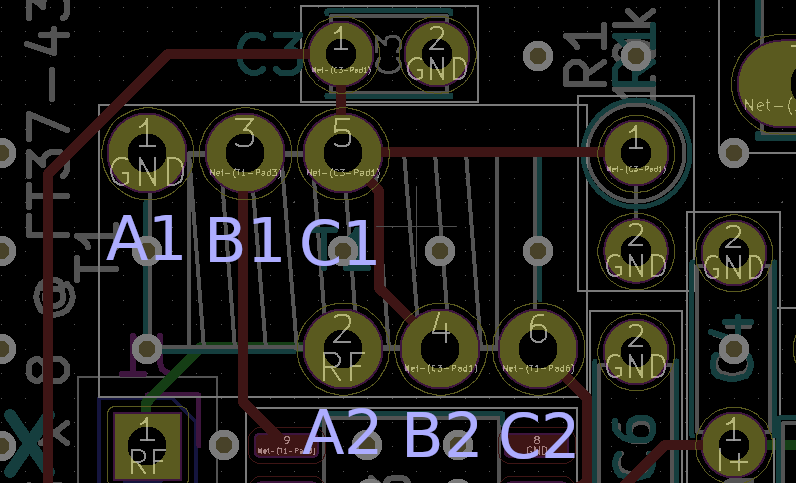
\includegraphics[width=0.9\textwidth]{fig/RX_T1.png}
   \caption{Footprint of T1}
 \end{subfigure}
 \begin{subfigure}[t]{0.49\textwidth}
   \centering
   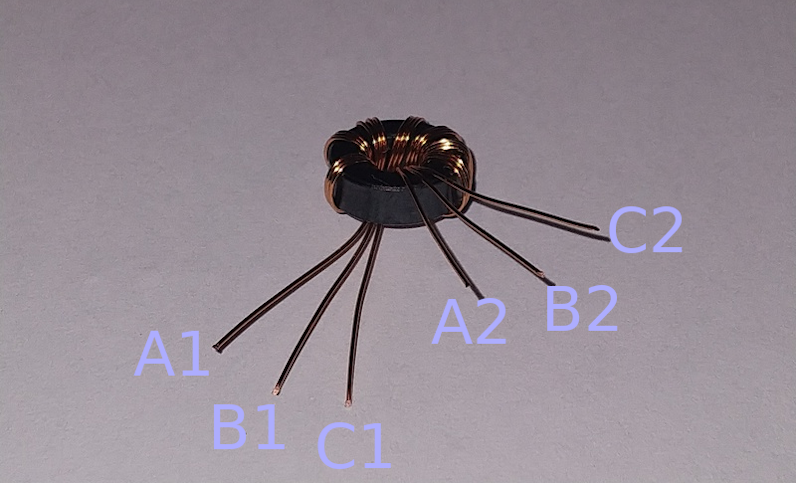
\includegraphics[width=0.9\textwidth]{fig/RX_T1_IMG_small.png}
   \caption{T1 wound and labeled.}
 \end{subfigure}
 \caption{Before soldering the core, make sure the wires are aligned correctly using a multi-meter. That is, top-left connects to bottom left (i.e., A1 to A2), top-center to bottom-center (i.e., B1 to B2) and top right to bottom right pads (i.e., C1 to C2) on the board.}
\end{figure}

\begin{warning}
The audio PA being used has a tendency to oscillate, in particular if a small speaker is used. If it does so, it may drive the complete audio-chain into saturation. In this case, the audio-chain may feed-back $12\,V$ to the FST3253 mixer. This may destroy the hard-to-get mixer! To prevent this problem, you \textbf{should} install four 5.1V Zener-diodes in parallel to C4-C7. This limits the voltage that can be fed back to the mixer and saves it. 
\end{warning}

\subsection{Receiver Test and Alignment}
Once the receiver is completed, re-connect the top-right pads \emph{+ G} to the power-supply, prepare the volume and head-phone plug. Also connect a piece of coaxial cable to the \emph{RX/GN} pads in the top-left. This is the antenna input for the test. Depending on the selected band, you may need to increase the current-limit of the power supply to about $120\,mA$. 

\subsubsection{Frequency Alignment}
If a accurate frequency-counter is at hand, you may start your alignment by fixing the PLL offset. Select the 20m band and tune to $14.0007 MHz$. Then measure the frequency at the USB pad. You should read exactly $14.000 MHz$ (if the CW side-tone frequency is set to $700\,Hz$). If not, enter the Setup menu and select the \emph{PLL correction} option. Now adjust the correction until you read $14.000 MHz$ in the frequency counter.

\subsubsection{CW Filter Alignment}
Although the CW filter cannot be \emph{tuned}, variations in component values may lead to small variations in the center frequency of the narrow CW audio filter. For a proper alignment of the RX frequency-shift, the CW-tone must be set to the center frequency of the CW filter. Hence, measure the spectrum (e.g., using your PC sound card and an application that can display the audio spectrum) of the audio signal. Determine the center frequency of the CW filter and set the CW side-tone frequency (under \texttt{Menu}\ $\rightarrow$\ \texttt{Setup}\ $\rightarrow$\ \texttt{CW Tone}) to that value. This will also adjust the RX frequency-shift.

\begin{remember}
The displayed frequency is the frequency, the TRX will transmit on. It is not the beat-frequency the TRX is receiving on.
\end{remember}

\subsubsection{Side-band Suppression}
If an signal generator is at hand, tune the generator to $14.000 MHz$. Then select the 20m Band and tune to $14.0012 MHz$. You may hear a low-frequency tone (about $500Hz$). Tune \texttt{RV2} \& \texttt{RV3} to minimize the unwanted side-band tone. Then tune to $14.0016 MHz$. You may hear a high-frequency tone (about $900 Hz$). Tune \texttt{RV1} \& \texttt{RV3} to minimize the unwanted side-band tone. You may repeat the previous steps several times to obtain the optimal result. In my experience, the unwanted side-band suppression will work satisfactorily on all bands once aligned properly on 20m. 

With these steps, the alignment of the RX is completed and you may take the RX on a short ride through the bands.

\clearpage
\subsection{RX Component List}  \label{sec:rxcomp}
\begin{longtable}{|l|p{6cm}|l|l|} \hline 
\# & Component & Value & Remarks \\ \hline 
1 & R15 & 10R & \\
4 & R20, R21, R22, R23 & 100R & \\
1 & R43 & 220R & \\
3 & R38, R39, R42 & 1k & \\
1 & R13 & 2.2k & \\
9 & R7, R27, R29-R31, R33, R35-R37 & 3.3k & \\
1 & R32 & 4.3k & \\
1 & R4 & 4.7k & \\
1 & R26 & 5.1k & \\
1 & R34 & 7.5k & \\
10 & R1, R2, R6, R11, R18, R24, R25, R28, R40, R41 & 10k & \\
2 & R9, R10 & 30k & \\
2 & R12, R14 & 33k & \\
2 & R16, R17 & 36k & \\
2 & R3, R5 & 47k & \\
1 & R8 & 120k & \\
1 & R19 & 470k & \\
2 & RV1, RV2 & 50k & \\
1 & RV3 & 500R & \\
1 & RV4 & 10k & \\
3 & C13, C20, C23 & 1n & \\
2 & C25, C27 & 3.3n & \\
3 & C30, C31, C35 & 10n & \\
5 & C12, C17, C18, C21, C33 & 47n & \\
23 & C3, C8, C11, C22, C24, C26, C29, C32, C34, C37-C41, C46-C54 & 100n & \\
5 & C4, C5, C6, C7, C36 & 470n & \\
2 & C1, C28 & 1u & \\
3 & C15, C16, C42 & 10u & \\
3 & C2, C14, C19 & 100u & \\
8 & L1, L3, L4, L5, L6, L7, L8, L9 & 100u & \\
1 & T1 & 3 x 8 @ FT37-43 & \\
1 & D1 & 1N4148 & \\
4 & in parallel to C1-C4 & 5.1V Zener & \\
1 & Q1 & BS170 & \\
1 & Q2 & 2N3904 & \\
1 & U1 & FST3253 & \\
5 & U3, U5, U6, U7, U8 & LM833 & \\
1 & U4 & LM386 & \\ 
6 & -- & DIP-8 Sockets & \\
1 & U9 & 74AC74 & \\
1 & U10 & L7805 & \\
1 & U11 & ATmega328-PU & \\
1 & --  & DIP-28 Socket & \\
1 & - & SI5351 break-out & \\
2 & J1, J3, J4, J11 & 1x10 pin-header long & \\
1 & J6 & 2x3 pin-header & \\
1 & J9 & 1x7 pin-socket & \\
2 & J2, J7 & 1x2 90deg & \\
1 & -- & Switch & \\
1 & J8 & 1x3 90deg & \\
1 & -- & 10k log & potentiometer \\
1 & J10 & 1x4 90deg & \\
1 & -- & Rotary encoder & \\
1 & LCD1 & 1x8 90deg & \\
1 & -- & LCD & 2 x 8 symbols \\
1 & J13 & TX-OC & RCA-jack (optional) \\
1 & J5 & Key & 3.5mm stereo jack\\ \hline
\end{longtable}


\cleardoublepage
\section{PA \& Low-Pass Board} \label{sec:pa}
The majority of the PA/LP board consists of four 7-pole Chebyshev low-pass filters. The Chebyshev-type filters are needed to get away with only four filters to cover all RF bands from 80m to 10m. The right-most filter covers the 80m and 60m band and should have a cutoff frequency near $5.6\,MHz$. The next filter covers 40m and 30m and should have a cutoff frequency near $10.5\,MHz$. The second-to-last filter covers 20m and 17m and should have a cutoff frequency near $20\,MHz$. Finally the leftmost filter will cover 15m, 12m and 10m with a cutoff frequency near $30\,MHz$. The low-pass filters are switched by 4 sub-miniature relays controlled by the RX-board via the board-to-board (b2b) connector \texttt{J2}.

The \texttt{Q4} mosfet acts as the TX/RX switch passing the LP-filtered RF from the input to the RX via b2b \texttt{J6}.

The PA section consist of a \texttt{74HCT00} as driver, four \texttt{BS170} mosfets as PA transistors and a \texttt{BD140-16} for key-shaping. The TX oscillator signal arrives from the RX-board via b2b \texttt{J7}.

The complete TRX is powered from the barrel-jack \texttt{J3} and the supply voltage is passed to the RX-board via b2b \texttt{J11}. 

\begin{remark}
 Before assembling the low-pass filers on the board. Please assemble them ugly-style on a piece of PCB material and measure their properties using a network analyzer or spectrum analyzer. Being Chebyshev low-pass filter, the exact component values are critical!
\end{remark}

 If no measurement equipment is present. Please subtract one winding from the given values below. The number of turns for each core was determined using AL-values provided by the manufacturer. In my experience, this leads to an slightly overestimation of the number of turns by about one. Moreover, you are probably more willing to risk a lower stop-band suppression rather than an increased damping in the pass band.

\begin{remark}
 Like for the RX board, the PA board has its own \href{https://dm3mat.darc.de/cw2019/pa_rev2_ibom.html}{interactive BOM}.
\end{remark}

 The diode \texttt{D4} is connected in parallel to the barrel-jack and acts together with a fuse as a reverse-polarity protection. If the supply is connected to the TRX in reverse-polarity, the diode will short the input which will cause a huge current that blows the fuse. A 2A \emph{flink} fuse will do.
 
 Finally install the b2b \textbf{sockets} on the PA/LP board, that is \texttt{J2}, \texttt{J6}, \texttt{J7} and \texttt{J11}.
 
\clearpage
\subsection{PA/LP Component List}  \label{sec:pacomp}
\begin{longtable}{|l|p{6cm}|l|l|} \hline 
\# & Component & Value & Remarks \\ \hline 
2 & R12, R13 & 100 & \\
1 & R9 & 470R & \\
1 & R10 & 1k & \\
1 & R14 & 4.7k & \\
7 & R1, R3, R5, R7, R11, R15, R16 & 10k & \\
4 & R2, R4, R6, R8 & 100k & \\
2 & C2, C15 & 100p & NP0 \\
4 & C3, C6, C11, C16 & 220p & NP0 \\
4 & C4, C7, C12, C17 & 470p & NP0 \\
2 & C5, C18 & 820p & NP0 \\
2 & C8, C13 & 1n & NP0 \\
2 & C9, C14 & 1.5n & NP0 \\
11 & C1, C10, C19, C20, C22, C23, C24, C27, C28, C29, C30 & 100n & \\
1 & C25 & 1u & \\
1 & C26 & 220u & \\
1 & L14 & 22u & 07HCP \\
1 & L13 & 100u & MICC \\
3 & L1, L5, L9 & 330n & 11T on T37-6 \\
3 & L2, L6, L10 & 480n & 13T on T37-6 \\
3 & L3, L7, L11 & 750n & 14T on T37-2 \\
3 & L4, L8, L12 & 1700n & 21T on T37-2 \\
1 & T1 & -- & 8T + 8T on FT37-43 \\
4 & K1, K2, K3, K4 & G6S-2 & \\
6 & D1, D2, D3, D5, D6, D7 & 1N4148 & \\
1 & D4 & 1N4001 & \\	
4 & Q1, Q2, Q3, Q10 & 2N3904 & \\
6 & Q4, Q6, Q7, Q8, Q9, Q11 & BS170 & \\
1 & Q5 & BD140-16 & \\
1 & U1 & 74HCT00 & \\
1 & J1 & BNC & \\
1 & J2 & 1 x 8 pin-socket & \\
1 & J3 & barrel-jack & \\
3 & J6, J7, J11 & 1 x 2 pin-socket & \\ \hline
\end{longtable}


\cleardoublepage
\section{Final Assembly} \label{sec:box}
Finally, the board-to-board interconnects are installed. The way these connectors are installed, depends on the chassis and distance between the boards you chose. The example I give here applies to the Fischer \texttt{KOH-2100} + \texttt{KOH-4100} + \texttt{DPL 2-4} kit. This is a nice and compact $10 \times 10 \times 5\,cm$ chassis. The boards slide into the chassis with $\approx 1.5\,cm$ distance. Unfortunately, I was not able to find stackers or long pin-headers with a matching length here in Germany. Have a look at Ebay or at Mouser. Pin headers with insertion lengths of about $12\,mm$ should do the trick. I, however, went with stackers of $38\,mm$ total length which is is way too long and therefore needed to be shortened.

\begin{figure}[!ht]
 \centering
 \begin{subfigure}{0.49\linewidth} 
  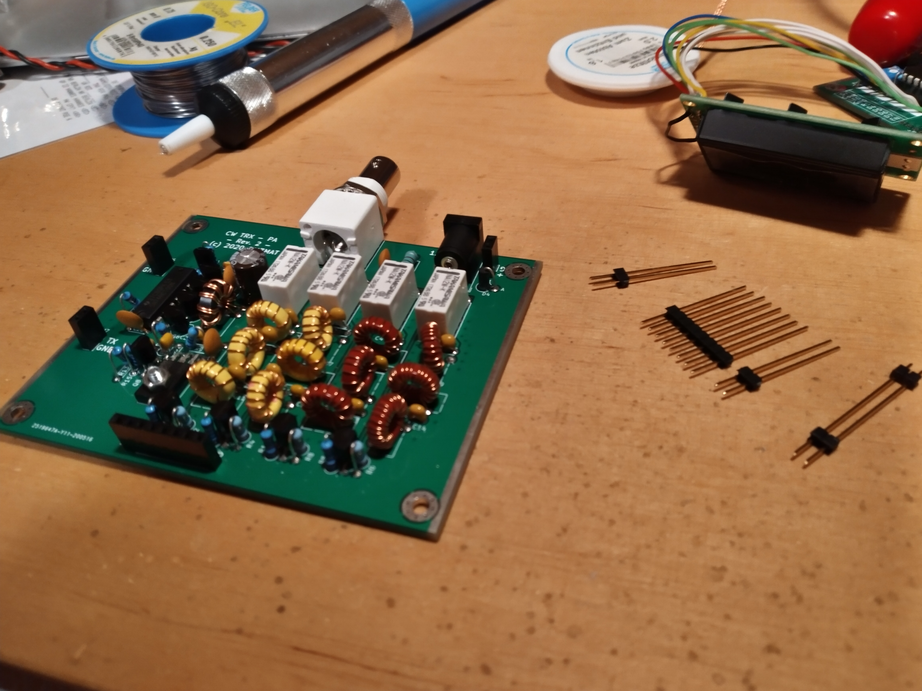
\includegraphics[width=\linewidth]{fig/stackers_small.png}
  \caption{Cut stackers to get long pin-headers, before inserting them into the socket of the PA board.} \label{fig:stackers}
 \end{subfigure} 
 \begin{subfigure}{0.49\linewidth} 
  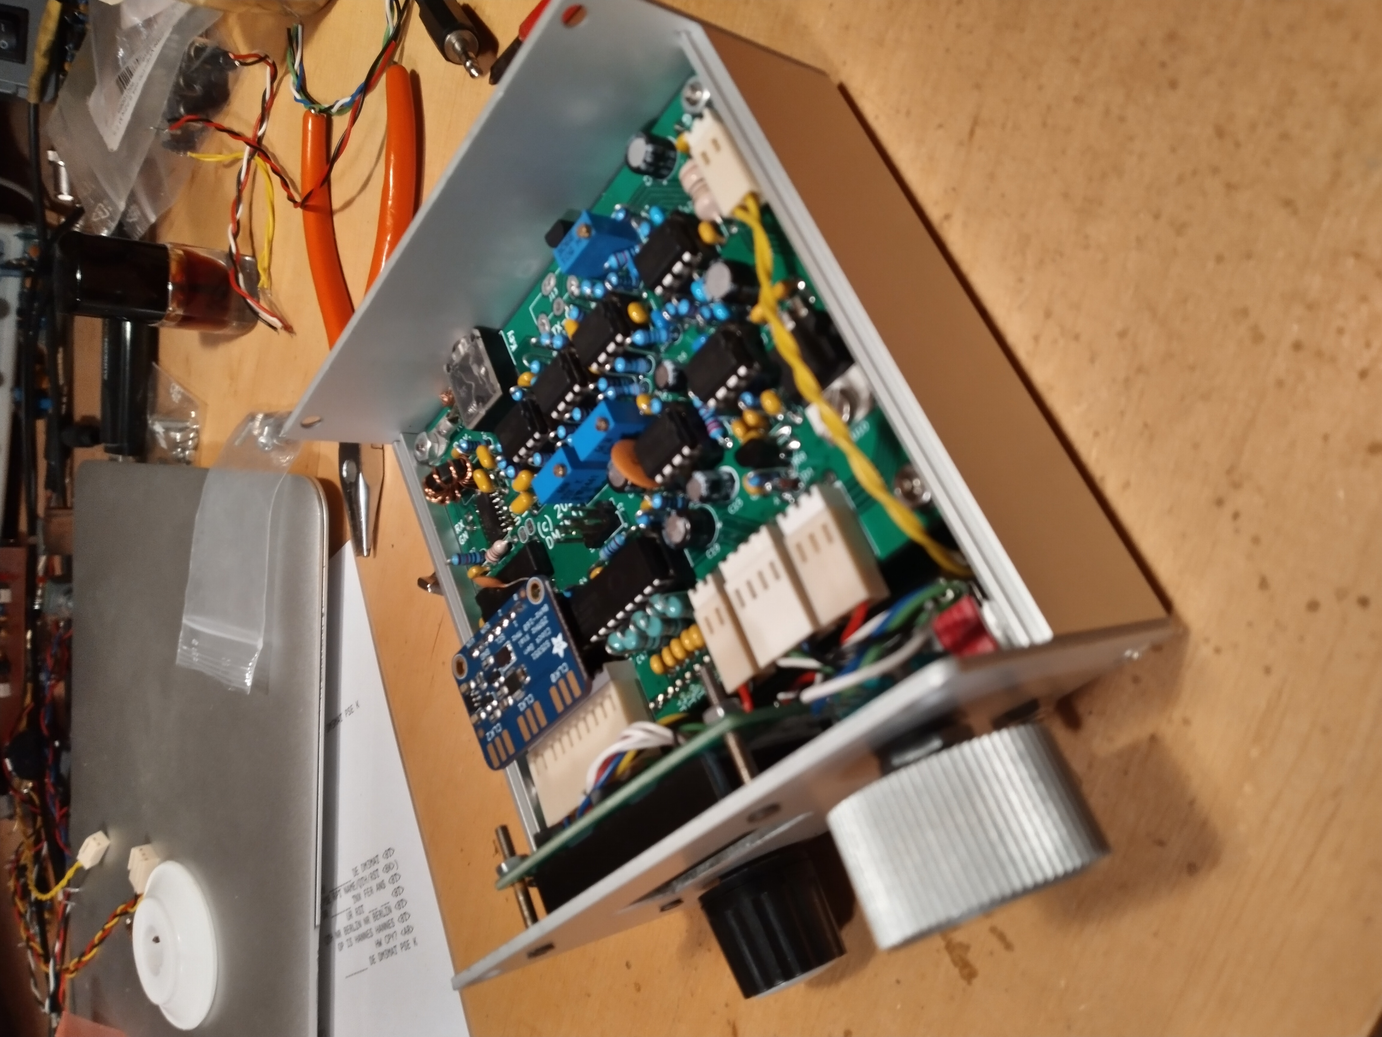
\includegraphics[width=\linewidth]{fig/final_small.png}
  \caption{Put RX board on top, insert into chassis, solder pins to RX board and cut pins to length.} \label{fig:final}
 \end{subfigure}
 \caption{Final assembly of the board-to-board interconnects.}
\end{figure}

The easiest way to do that, is to cut the top-part away from these stackers (see figure \ref{fig:stackers}) and stick them into the sockets on the PA board. Than put the RX board on top. Now carefully insert both boards in the chassis. Make sure that you can close the chassis. Finally solder the stackers/long pin-headers into the RX board. 

\begin{warning}
Do not overheat the stackers/pin-headers as the socket may melt. Just tag them in-place and reflow the header connections once the PA-board is removed.
\end{warning}

When the TRX is installed into the Fischer chassis mentioned above, the RCA connector at the back of the RX board to key an external PA will not fit. The boards are way to close together. If a different chassis is used, the connector can be installed right now.


\subsection{Final Testing}
With these final steps completed, it is now time to test the PA and RX/TX switching. Reconnect everything and connect a dummy-load to the output. Measure the RF voltage-drop across the dummy-load (oscilloscope). Alternatively, connect a power/SWR meter between the TRX and dummy-load. You should get about $22\,Vp$ across the dummy-load or about $5\,W$ on transmit, depending on the supply voltage (assuming about $13.8\,V$). On the lower band (e.g., up to $30\,m$) it might even be a little bit more. 

If your output is way less, measure the peak voltages at the PA-output and LP-input and double-check the low-pass filters. If the output matches, the assembly is complete. 

\subsection{Hot fixes}
The second revision was a redesign to some extend. Hence not everything is perfect yet. For example, the \texttt{74AC74} produces a lot of high-frequency ripple on the 5V rail. To suppress them stronger, a $470\,pF$ capacitor should be soldered directly from pin 16 (5V) to pin 8 (GND).  

The audio PA has a tendency to oscillate, in particular if a small speaker is used. If it does so, it may drive the complete audio-chain into saturation. In this case, the audio-chain may feed-back $12\,V$ to the FST3253 mixer. This destroys the hard-to-get mixer! To prevent this problem, you \textbf{should} install four 5.1V Zener-diodes in parallel to C4-C7 on the receiver board. This limits the voltage that can be fed back to the mixer and saves it. 

\subsection{Mechanical Parts}
\begin{longtable}{|l|p{6cm}|l|l|} \hline 
\# & Component & Remarks \\ \hline 
1 & chassis top & \\
1 & chassis bottom & \\
1 & chassis front/back & \\
1 & 10k log pot & \\
1 & rotary encoder & \\
1 & LCD display & \\
1 & head-phone socket & \\
1 & switch & \\
1 & barrel plug & \\
2 & fuse holder & optional \\
2 & 2A flink & optional \\
1 & speaker & optional \\ \hline
\end{longtable}


\cleardoublepage 
\section{Build \& Load the Firmware} \label{sec:fw}
To program the firmware onto the device in the first place or update the firmware to a newer version, a so-called in-system programmer ISP is needed. This is a small USB device that provides the interface from the computer to the controller (MCU). There are many cheap AVR ISPs out there (usually between 5\EUR and 10\EUR on ebay). It is also possible to build a \href{http://www.lancos.com/siprogsch.html}{makeshift ISP for the good old serial-port} or using a \href{https://www.arduino.cc/en/Tutorial/BuiltInExamples/ArduinoISP}{Arduino as ISP}. 

Once you got your hands on an ISP, you still need some software to upload the firmware to the device. I used \href{https://www.nongnu.org/avrdude/}{avrdude} under Linux for this but others should work as well. If you got a working setup, you can simply \href{https://github.com/hmatuschek/cwtrx/releases}{download} the pre-compiled firmware and EEPROM image from my github page and program the device immediately. You only need to set the fuses of the AtMega first to low=\texttt{0xE2} and high=\texttt{0xD9}. These fuse settings tells the MCU to use the internal 8Mhz RC-oscillator (no pins left for a crystal) and not to divide the clock by 8. All other settings are left as default. 

\begin{wrapfigure}{l}{0.2\linewidth}
  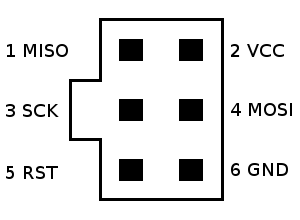
\includegraphics[width=\linewidth]{fig/icsp_6pin.png}
\end{wrapfigure}
You can find the 6-pin ISP header (J3) on the RX board. Pin 1 is marked by a small circle on the corner. Consequently the small tab on the ISP plug must face away from the MCU. 

When programming the MCU, you need to first set the fuses. This step must only be done once as these settings are conserved across programming cycles. In a second step the firmware (\texttt{firmware-atmega328p.hex}) is written to the MCU. This step usually erases the EEPROM content. The EEPROM is used to store settings, last frequency etc. The firmware may not properly work with some uninitialized EEPROM. Hence, after the firmware was written, the default EEPROM image (\texttt{firmware-atmega328p-eeprom.hex}) must be written to the MCU.

\subsection{Building Firmware from Scratch}
In this section, I like to describe building and loading the firmware from scratch on a Ubuntu/Debian system (e.g., on a Raspberry Pi). Before you can start a bunch of software needs to be installed. That is the cross compiler, build tools and programming software. So run on a command line
\begin{lstlisting}[language=bash]
sudo apt-get install git cmake gcc-avr avrdude
\end{lstlisting}

\texttt{git} is the version control system I use. It is used to download the latest source code. \texttt{cmake} is the build system. There is a nice extension to cmake for the avr-gcc and avrdude that makes building and writing the firmware to the MCU easy. \texttt{gcc-avr} is the cross-compiler for the AVR devices. Finally, \texttt{avrdude} is the programming tool to write the firmware to the device.

Once all the software is installed, you need to download the firmware source from my github page. So call
\begin{lstlisting}[language=bash]
git clone https://github.com/hmatuschek/cwtrx.git
\end{lstlisting}
You will now find a new directory named \texttt{cwtrx}. Before the firmware can be programmed to the device, you may need to adjust some settings to reflect your programmer. The first lines in the \texttt{cwtrx/\-firmware/\-CMakeLists.txt} specify which programmer you use and where to find it. 

By default you should find something like this
\lstinputlisting[linerange={1-4}, numbers=left]{../firmware/CMakeLists.txt}
In the second line, you can set the programming tool. Here avrdude is used. The third line specifies the ISP programmer being used. Here I used a STK500V2 compatible one (actually called DIAMEX-AVR). Finally, line 4 specifies the port where the programmer can be found. This programmer appears as a serial port to the computer (as device \texttt{/dev/ttyACM0}). You may need to change lines 3 and 4 to match your local setup.

Once everything is set up, you can start to build the firmware. Enter the \texttt{cwtrx} directory, create a so-called build directory and enter it as well. 
\begin{lstlisting}[language=bash]
cd cwtrx
mkdir build
cd build
\end{lstlisting}

In the next step, the build will be configured with
\begin{lstlisting}[language=bash]
cmake ..
\end{lstlisting}
This step will search for the AVR GCC and prepare the build. Once completed, build the firmware and EEPROM image with
\begin{lstlisting}[language=bash]
make
\end{lstlisting}

After this step, you need to set the fuses of the MCU. Simply call
\begin{lstlisting}[language=bash]
make set_fuses
\end{lstlisting}
This step may fail if the MCU is brand new. Just retry several times. Once the fuses are set, the communication with the MCU should be stable. Then upload the firmware to the MCU with
\begin{lstlisting}[language=bash]
make upload_firmware
\end{lstlisting}
and finally write the EEPROM image with 
\begin{lstlisting}[language=bash]
make upload_eeprom
\end{lstlisting}

Your TRX is now ready.

\subsection{Updating the Firmware}
Assuming you already performed the steps above, updating the firmware is quiet straight forward. Enter the \texttt{cwtrx} directory and run
\begin{lstlisting}[language=bash]
git pull
cd build
make 
make upload_firmware
make upload_eeprom
\end{lstlisting}
And you are ready to go.


\cleardoublepage
\section{Usage} \label{sec:user}
Handling a feature-rich TRX using a single rotary encoder with a single push-button is kind of challenging. I've designed a two-level menu navigation that puts everything that is needed frequently in the first level (blue in figure \ref{fig:menu}) and everything else in a second level. This keeps the navigation fast for frequently used options. 

The second menu level (red in figure \ref{fig:menu}) contains all settings that are usually not touched during the operation. They concern the basic setup and alignment of the TRX. 

\begin{figure}[!ht]
 \centering
 \footnotesize
 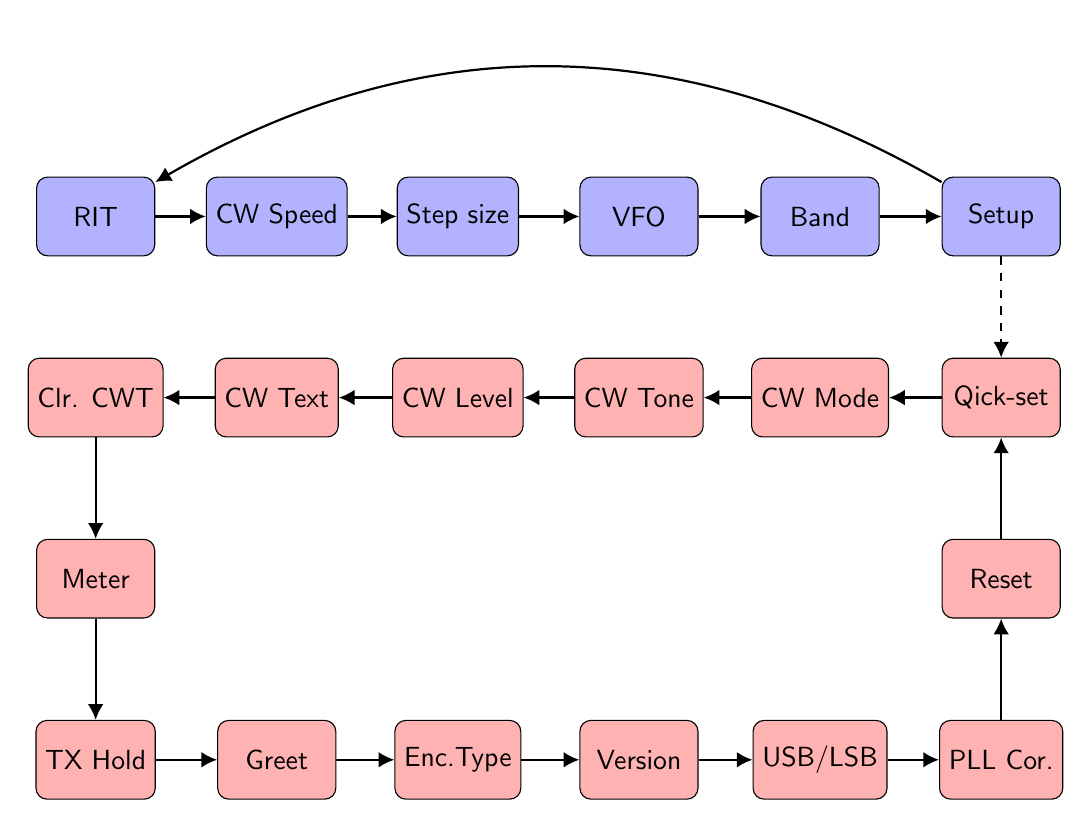
\begin{tikzpicture}[node distance=2.3cm,
	>={Latex[width=2mm,length=2mm]},
    menu/.style = {rectangle, rounded corners, draw=black,
                   minimum width=1.5cm, minimum height=1cm,
                   text centered, font=\sffamily, fill=blue!30},
    submenu/.style = {menu, fill=red!30}]
  \node (rit) [menu] {RIT};   
  \node (speed) [menu, right of=rit] {CW Speed}; 
  \node (step) [menu, right of=speed]{Step size};
  \node (vfo) [menu, right of=step] {VFO};
  \node (band) [menu, right of=vfo] {Band};
  \node (setup) [menu, right of=band] {Setup};
  
  \node (quick) [submenu, below of=setup] {Qick-set};
  \node (cw) [submenu, left of=quick] {CW Mode}; 
  \node (tone) [submenu, left of=cw] {CW Tone}; 
  \node (level) [submenu, left of=tone] {CW Level}; 
  \node (text) [submenu, left of=level] {CW Text}; 
  \node (clr) [submenu, left of=text] {Clr. CWT};
  \node (meter) [submenu, below of=clr] {Meter};
  \node (hold) [submenu, below of=meter] {TX Hold}; 
  \node (greet) [submenu, right of=hold] {Greet};
  \node (enc) [submenu, right of=greet] {Enc.Type};
  \node (version) [submenu, right of=enc] {Version};
  \node (sideband) [submenu, right of=version] {USB/LSB};
  \node (pll) [submenu, right of=sideband] {PLL Cor.};
  \node (reset) [submenu, above of=pll] {Reset};
  
  
  \path[->,thick]
    (rit) edge (speed)
    (speed) edge (step)
	(step) edge (vfo)
	(vfo) edge (band)
	(band) edge (setup)
	(setup) edge[bend right] (rit);
	
  \path[->,thick,dashed]
    (setup) edge (quick);
  \path[->,thick]
        (quick) edge (cw)
    	(cw) edge (tone)
    	(tone) edge (level) 
    	(level) edge (text)
    	(text) edge (clr)
    	(clr) edge (meter) 
    	(meter) edge (hold)
    	(hold) edge (greet) 
    	(greet) edge (enc)
    	(enc) edge (version)
    	(version) edge (sideband)
    	(sideband) edge (pll)
    	(pll) edge (reset) 
    	(reset) edge (quick);
 \end{tikzpicture}
 \caption{Menu navigation} \label{fig:menu}
\end{figure}

To enter the menu, just click the button on the rotary encoder. You will land on either the RIT setting or on the last modified setting. Using the rotary-encoder you can navigate through the first menu level. To change a settings, click the center button again. You can now change the selected setting using the rotary encoder. To finish the setting and leave the menu, click the center button again.

To enter the second menu-level, enter the first level by clicking on the center button and select the menu entry \texttt{Setup}. Click on the center button again to enter the second-level menu. You will land on the \texttt{Quick-set} setting. You may now navigate the second menu-level using the rotary encoder. Changing and leaving the second-level menu works in the same way as the first-level menu. 


\subsection{Gestures}
The firmware distinguishes four different \emph{gestures} of the rotary encoder:
\begin{enumerate}
 \item \emph{tune} - just rotate the encoder.
 \item \emph{click} - press and release the center button of the encoder.
 \item \emph{long-press} - press and hold the center button for at least 2 seconds.
 \item \emph{press-rotate} - press and rotate the encoder.
\end{enumerate}

During RX, a \emph{tune} gesture will simply tune the frequency (of cause), a \emph{click} gesture will enter the menu, a \emph{long-press} gesture will send the keyer memory (if set) and a \emph{press-rotate} gesture will quick-set a property (if specified).


\subsection{Settings}
The \emph{settings} are all settings that might be changed during normal operation of the TRX. Hence they are located at the first level of the menu for the sake of quick access.
 
\paragraph{Receive/Transmit offset (RIT)}
Allows to fine-tune the RX frequency while keeping the TX frequency constant. A non-zero RIT will be indicated by a \texttt{+} or \texttt{-} symbol in the bottom-right corner of the display during RX. 

\paragraph{CW speed}
Specifies the speed in WPM for the iambic and automatic keyer.

\paragraph{Tuning step-size}
Specifies the step-size when tuning the TRX.

\paragraph{VFO}
Specifies the current VFO and VFO-mode. That is \texttt{VFO A}, \texttt{VFO B} or \texttt{Split}.

\paragraph{Band}
Specifies the current band. 


\subsection{Quick-Set}
The \emph{quick-set} feature allows you to modify a selected setting without entering the menu at all. Just press \& rotate the  encoder.

To use this feature, you have to specify the settings you want to \emph{quick-set} under \texttt{Menu} $\rightarrow$ \texttt{Setup} $\rightarrow$ \texttt{QuickSet} (see below).

\subsection{Setup}
\emph{Setup} hides all settings that are usually not touched during regular operation and are therefore hidden in the second menu-level. You can access these settings by selecting \texttt{Menu} $\rightarrow$ \texttt{Setup}.

\paragraph{Quick-set}
The quick-set feature allows to set a specific property without entering the menu. By holding and turning the rotary-encoder at the same time. This menu item allows to select one of four settings to be manipulated by the quick-set feature: RIT, keyer speed, tuning step-size, band or \emph{none}. The latter disables the quick-set feature (default).

\paragraph{Keyer mode}
The keyer mode specifies the type of keyer you use. Possible options are \emph{straight key} and \emph{iambic}. The TRX switches automatically to \emph{straight key} if the TRX detects a mono-plug at startup.

\paragraph{CW side-tone level}
Specifies the volume of the CW side-tone. This is a value between 1 and 255.

\paragraph{Keyer memory \texttt{CW Text}}
Specifies the text to be send automatically (e.g., a CQ call) when the rotary encoder is long-pressed. If no text is set, nothing will happen.

To edit the CW text head to \texttt{Menu} $\rightarrow$ \texttt{Setup} $\rightarrow$ \texttt{CW Text} and \emph{click} the encoder to enter the editor. You should see a cursor beneath the first character. You can use the encoder to select the character you want to edit. \emph{Click} again and the character should start to blink. You can now change the selected character. Once the desired character is found, \emph{click} again to set it. You are now back at the editor level and the next character is automatically selected. Once the text is edited, leave the editor by \emph{long-pressing} the encoder.

\paragraph{Clear keyer memory}
Simply clears the keyer memory.

\paragraph{Meter selection}
Selects a meter to display during RX. This can be \texttt{Volt} to display the supply voltage or \texttt{Temp} to display the core-temperature of the MCU.

\paragraph{TX-hold time}
Specifies the delay between TX and RX in $ms$. By default a value of $50\,ms$ is selected. This small value allows for quasi-QSK but is sufficiently long to avoid ugly clicks in the audio path when switching from TX to RX.
\begin{remark}
When operating a PA or in split mode, a longer delay should be chosen to allow the relays to switch properly.
\end{remark}

\paragraph{Greet text}
An editor that allows you to change the \emph{greeting} at startup. The editing is similar to the \emph{keyer memory} editor above.


\subsection{Alignment}
These settings can be found under the \emph{Setup} sub-menu and are usually only changed during the alignment of the TRX. 

\paragraph{CW side-tone frequency}
Specifies the CW side-tone frequency as well as the RX frequency shift. This frequency should be identical to the center frequency of the narrow CW audio filter.

\paragraph{Encoder type}
Specifies the encoder type used. There are two different generic encoder-types \texttt{A} \& \texttt{B}. If you ordered exactly the encoder listed in the BOM, you should have a type-A encoder (default). If you encounter problems with the encoder (e.g., double-steps) you may change this setting to type B. If you wired the encoder in the wrong way (wrong tuning direction) you may simply change this setting to \texttt{A~rev} or \texttt{B~rev}. 

\paragraph{PLL correction}
This setting specifies the PLL clock frequency correction in PPM. See \texttt{RX Alignment} above.

\paragraph{Factory reset}
The previous version of the TRX encountered some issues with the EEPROM memory, leading to corrupted settings which turn the TRX unusable. This option allows to reset the entire EEPROM memory to \emph{factory settings} fixing the corrupted memory issue.



\cleardoublepage
\section{Bill-of-Material (BOM)}
\begin{longtable}{|p{0.02\textwidth}|p{0.02\textwidth}|p{0.3\textwidth}|p{0.3\textwidth}|p{0.07\textwidth}|p{0.07\textwidth}|}\hline
\# & & Value & Reichelt & Cost & Sum \\ \hline\hline
1 & $\square$ & 10R & METALL 10,0 & 0,05 \euro & 0,05 \euro \\
6 & $\square$ & 100R & METALL 100 & 0,05 \euro & 0,29 \euro \\
1 & $\square$ & 220R & METALL 220 & 0,05 \euro & 0,05 \euro \\ 
1 & $\square$ & 470R & METALL 470 & 0,05 \euro & 0,05 \euro \\
4 & $\square$ & 1k & METALL 1,00K & 0,05 \euro & 0,20 \euro \\
1 & $\square$ & 2.2k & METALL 2,20K & 0,05 \euro & 0,05 \euro \\
9 & $\square$ & 3.3k & METALL 3,30K & 0,05 \euro & 0,44 \euro \\
1 & $\square$ & 4.3k & METALL 4,30K & 0,05 \euro & 0,05 \euro \\
2 & $\square$ & 4.7k & METALL 4,70K & 0,05 \euro & 0,10 \euro \\
1 & $\square$ & 5.1k & METALL 5,10K & 0,05 \euro & 0,05 \euro \\
1 & $\square$ & 7.5k & METALL 7,50K & 0,05 \euro & 0,05 \euro \\
17 & $\square$ & 10k & METALL 10,0K & 0,05 \euro & 0,83 \euro \\
2 & $\square$ & 30k & METALL 30,0K & 0,05 \euro & 0,10 \euro \\
2 & $\square$ & 33k & METALL 33,0K & 0,05 \euro & 0,10 \euro \\
2 & $\square$ & 36k & METALL 36,0K & 0,05 \euro & 0,10 \euro \\
2 & $\square$ & 47k & METALL 47,0K & 0,05 \euro & 0,10 \euro \\
4 & $\square$ & 100k & METALL 100K & 0,05 \euro & 0,20 \euro \\
1 & $\square$ & 120k & METALL 120K & 0,05 \euro & 0,05 \euro \\
1 & $\square$ & 470k & METALL 470K & 0,05 \euro & 0,05 \euro \\
2 & $\square$ & 50k & 64W-50K & 0,31 \euro & 0,62 \euro \\
1 & $\square$ & 500R & 64W-500 & 0,27 \euro & 0,27 \euro \\
1 & $\square$ & 10k & ACP 6-L 10K & 0,21 \euro & 0,21 \euro \\ \hline
2 & $\square$ & 100p & NPO-2,5 100P & 0,07 \euro & 0,14 \euro \\
4 & $\square$ & 220p & NPO-2,5 220P & 0,08 \euro & 0,32 \euro \\
4 & $\square$ & 470p & NPO-2,5 470P & 0,09 \euro & 0,36 \euro \\
2 & $\square$ & 820p & Conrad: 1578706 & 0,16 \euro & 0,32 \euro \\
3 & $\square$ & 1n & X7R-2,5 1,0N & 0,07 \euro & 0,21 \euro \\
2 & $\square$ & 1n & NPO-2,5 1,0N & 0,09 \euro & 0,18 \euro \\
2 & $\square$ & 1.5n & X7R-2,5 1,5N & 0,07 \euro & 0,14 \euro \\
2 & $\square$ & 3.3n & X7R-2,5 3,3N & 0,07 \euro & 0,14 \euro \\
3 & $\square$ & 10n & X7R-2,5 10N & 0,07 \euro & 0,21 \euro \\
5 & $\square$ & 47n & X7R-2,5 47N & 0,11 \euro & 0,55 \euro \\
35 & $\square$ & 100n & Z5U-2,5 100N & 0,05 \euro & 1,75 \euro \\
5 & $\square$ & 470n & Z5U-5 470N & 0,19 \euro & 0,95 \euro \\
3 & $\square$ & 1u & Z5U-5 1,0µ & 0,26 \euro & 0,78 \euro \\ \hline		
3 & $\square$ & 10u & RAD 10/35 & 0,02 \euro & 0,06 \euro \\
3 & $\square$ & 100u & RAD 100/16 & 0,03 \euro & 0,09 \euro \\
1 & $\square$ & 220u & RND 150ECR AY & 0,06 \euro & 0,06 \euro \\ \hline
1 & $\square$ & 22u & L-07HCP 22µ & 0,38 \euro & 0,38 \euro \\
9 & $\square$ & 100u & L-MICC 100µ & 0,27 \euro & 2,43 \euro \\ \hline
2 & $\square$ & FT37-43 & FT 37-43 & 0,58 \euro & 1,16 \euro \\
6 & $\square$ & T 37-6 & T 37-6 & 0,78 \euro & 4,68 \euro \\
6 & $\square$ & T 37-2 & T 37-2 & 0,54 \euro & 3,24 \euro \\ \hline
7 & $\square$ & 1N4148 & 1N 4148 & 0,02 \euro & 0,14 \euro \\
1 & $\square$ & 1N4001 & 1N 4001 & 0,02 \euro & 0,02 \euro \\
4 & $\square$ & 5.1V Zener & RND 1N751A &0,02 \euro & 0,08 \euro \\
7 & $\square$ & BS170 & BS 170 & 0,10 \euro & 0,70 \euro \\
5 & $\square$ & 2N3904 & 2N 3904 & 0,04 \euro & 0,20 \euro \\
1 & $\square$ & BD140 & BD 140-16 STM & 0,19 \euro & 0,19 \euro \\
1 & $\square$ & FST3253 & SOIC-16, Ebay & 2,00 \euro & 2,00 \euro \\
5 & $\square$ & LM833 & LM 833 & 0,90 \euro & 4,50 \euro \\
1 & $\square$ & LM386 & LM 386 DIP & 0,22 \euro & 0,22 \euro \\
6 & $\square$ & DIP-8 socket (optional) & GS 8 & 0,04 \euro & 0,24 \euro \\
1 & $\square$ & 74AC74 & Kessler: 522421 & 0,36 \euro & 0,36 \euro \\
1 & $\square$ & 74HCT00 & 74HCT 00 & 0,33 \euro & 0,33 \euro \\
1 & $\square$ & L7805 & L 7805 CV & 0,25 \euro & 0,25 \euro \\
1 & $\square$ & ATmega328-PU & ATMEGA 328P-PU & 2,50 \euro & 2,50 \euro \\
1 & $\square$ & DIP-28 socket (optional) & GS 28-S & 0,10 \euro & 0,10 \euro \\
1 & $\square$ & SI5351 breakout & Adafruit & 7,35 \euro & 7,35 \euro \\ \hline
4 & $\square$ & G6S-2 & NA 12W K & 0,96 \euro & 3,84 \euro \\ \hline
2 & $\square$ & 1x10 pin-header long & STAPELLEISTE 10 & 0,38 \euro & 0,76 \euro \\
1 & $\square$ & 2x3 pin-header & MPE 087-2-006 & 0,14 \euro & 0,14 \euro \\
1 & $\square$ & 1x7 pin-socket & MPE 156-1-007 & 0,37 \euro & 0,27 \euro \\
2 & $\square$ & 1x2 90deg & PSS 254/2W & 0,02 \euro & 0,04 \euro \\
2 & $\square$ & 1x2 plug & PSK 254/2W & 0,02 \euro & 0,04 \euro \\
1 & $\square$ & 1x3 90deg & PSS 254/3W & 0,04 \euro & 0,04 \euro \\
1 & $\square$ & 1x3 plug & PSK 254/3W & 0,02 \euro & 0,02 \euro \\
1 & $\square$ & 1x4 90deg & PSS 254/4W & 0,09 \euro & 0,09 \euro \\
1 & $\square$ & 1x4 plug & PSK 254/4W & 0,02 \euro & 0,02 \euro \\
1 & $\square$ & 1x10 90deg & PSS 254/10W & 0,10 \euro & 0,10 \euro \\
1 & $\square$ & 1x10 plug & PSK 254/10W & 0,08 \euro & 0,08 \euro \\
2 & $\square$ & contacts & PSK-KONTAKTE & 0,29 \euro & 0,58 \euro \\
2 & $\square$ & head-phone socket & EBS 35 & 0,30 \euro & 0,60 \euro\\
1 & $\square$ & TX-OC & CBP & 0,21 \euro & 0,21 \euro \\
1 & $\square$ & BNC & UG 1094W1 & 0,99 \euro & 0,99 \euro \\
1 & $\square$ & 1 x 8 socket & MPE 094-1-008 & 0,24 \euro & 0,14 \euro \\
1 & $\square$ & barrel jack & DC BU21 90 & 0,46 \euro & 0,46 \euro \\
3 & $\square$ & 1 x 2 socket & RND 205-00642 & 0,02 \euro & 0,06 \euro \\ \hline
1 & $\square$ & chassis top & KOH-2100 & 5,40 \euro & 5,40 \euro \\
1 & $\square$ & chassis bottom & KOH-4100 & 5,80 \euro & 5,80 \euro \\
1 & $\square$ & chassis front/back & DPL 2-4 & 7,99 \euro & 7,99 \euro \\
1 & $\square$ & 10k log pot & RK11K112-LOG10K & 1,35 \euro & 1,35 \euro \\
1 & $\square$ & rotary encoder & STEC11B03 & 3,70 \euro & 3,70 \euro \\
1 & $\square$ & LCD display & LCD-PM 2X8-5 A & 7,30 \euro & 7,30 \euro \\
1 & $\square$ & switch & KIPP 1A11 & 1,20 \euro & 1,20 \euro \\
1 & $\square$ & barrel plug & HS 21-13 & 0,20 \euro & 0,20 \euro \\
2 & $\square$ & fuse holder (optional) & RND 170-00170 & 0,19 \euro & 0,38 \euro \\
2 & $\square$ & 2A flink (optional) & ESKA 520.020 & 0,09 \euro & 0,18 \euro \\
1 & $\square$ & speaker (optional) & LSM-S20K & 2,70 \euro & 2,70 \euro \\ \hline \hline
\multicolumn{4}{|l}{Total\footnote{Prices may change over time.}} & \multicolumn{2}{r|}{\textbf{89,21 \euro}} \\ \hline
\end{longtable}


\subsection{Shave off some \euro\ from the BOM}
The single most expensive item on the BOM is the chasis. You can certainly find some extruded aluminium chassis for less than \EUR{5} on Ebay. You can also get cheap clones of the Adafruit SI5351 break-out board for around \EUR{3}, cheap rotary encoders (\EUR{1}) and 2x8 LCD displays (\EUR{3}) there. I shoud announce a competition for the cheapest BOM for this TRX.

\cleardoublepage
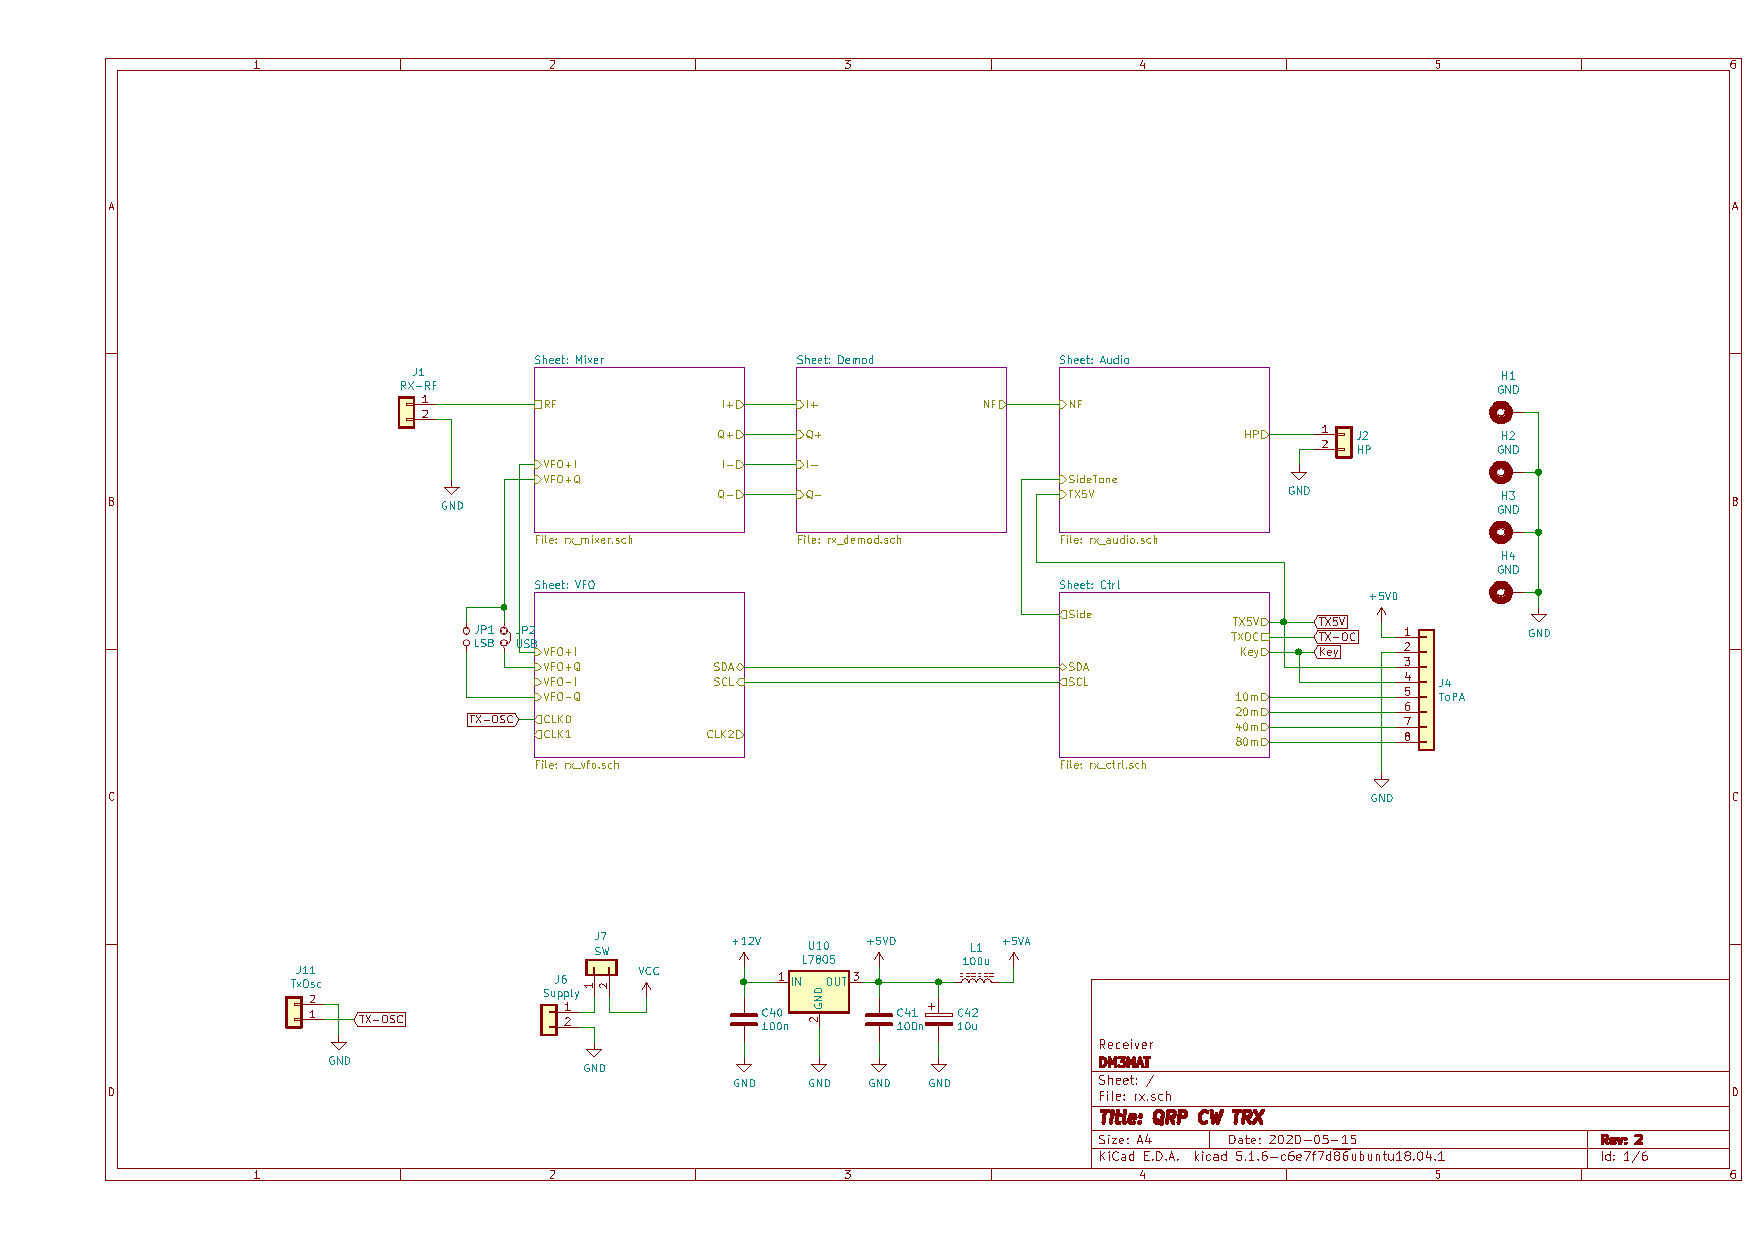
\includepdf[pages={1,2,4,3,5,6},landscape=true, addtotoc={
 1, section, 1, RX Circuit, rxscm,
 2, subsection, 1, RX Mixer, rxmix,
 4, subsection, 1, Demodulator, rxdemod,
 3, subsection, 1, AF-Section, rxaudio,
 5, subsection, 1, PLL, rxpll,
 6, subsection, 1, Controller, rxctrl}]{fig/rx_scm.pdf}
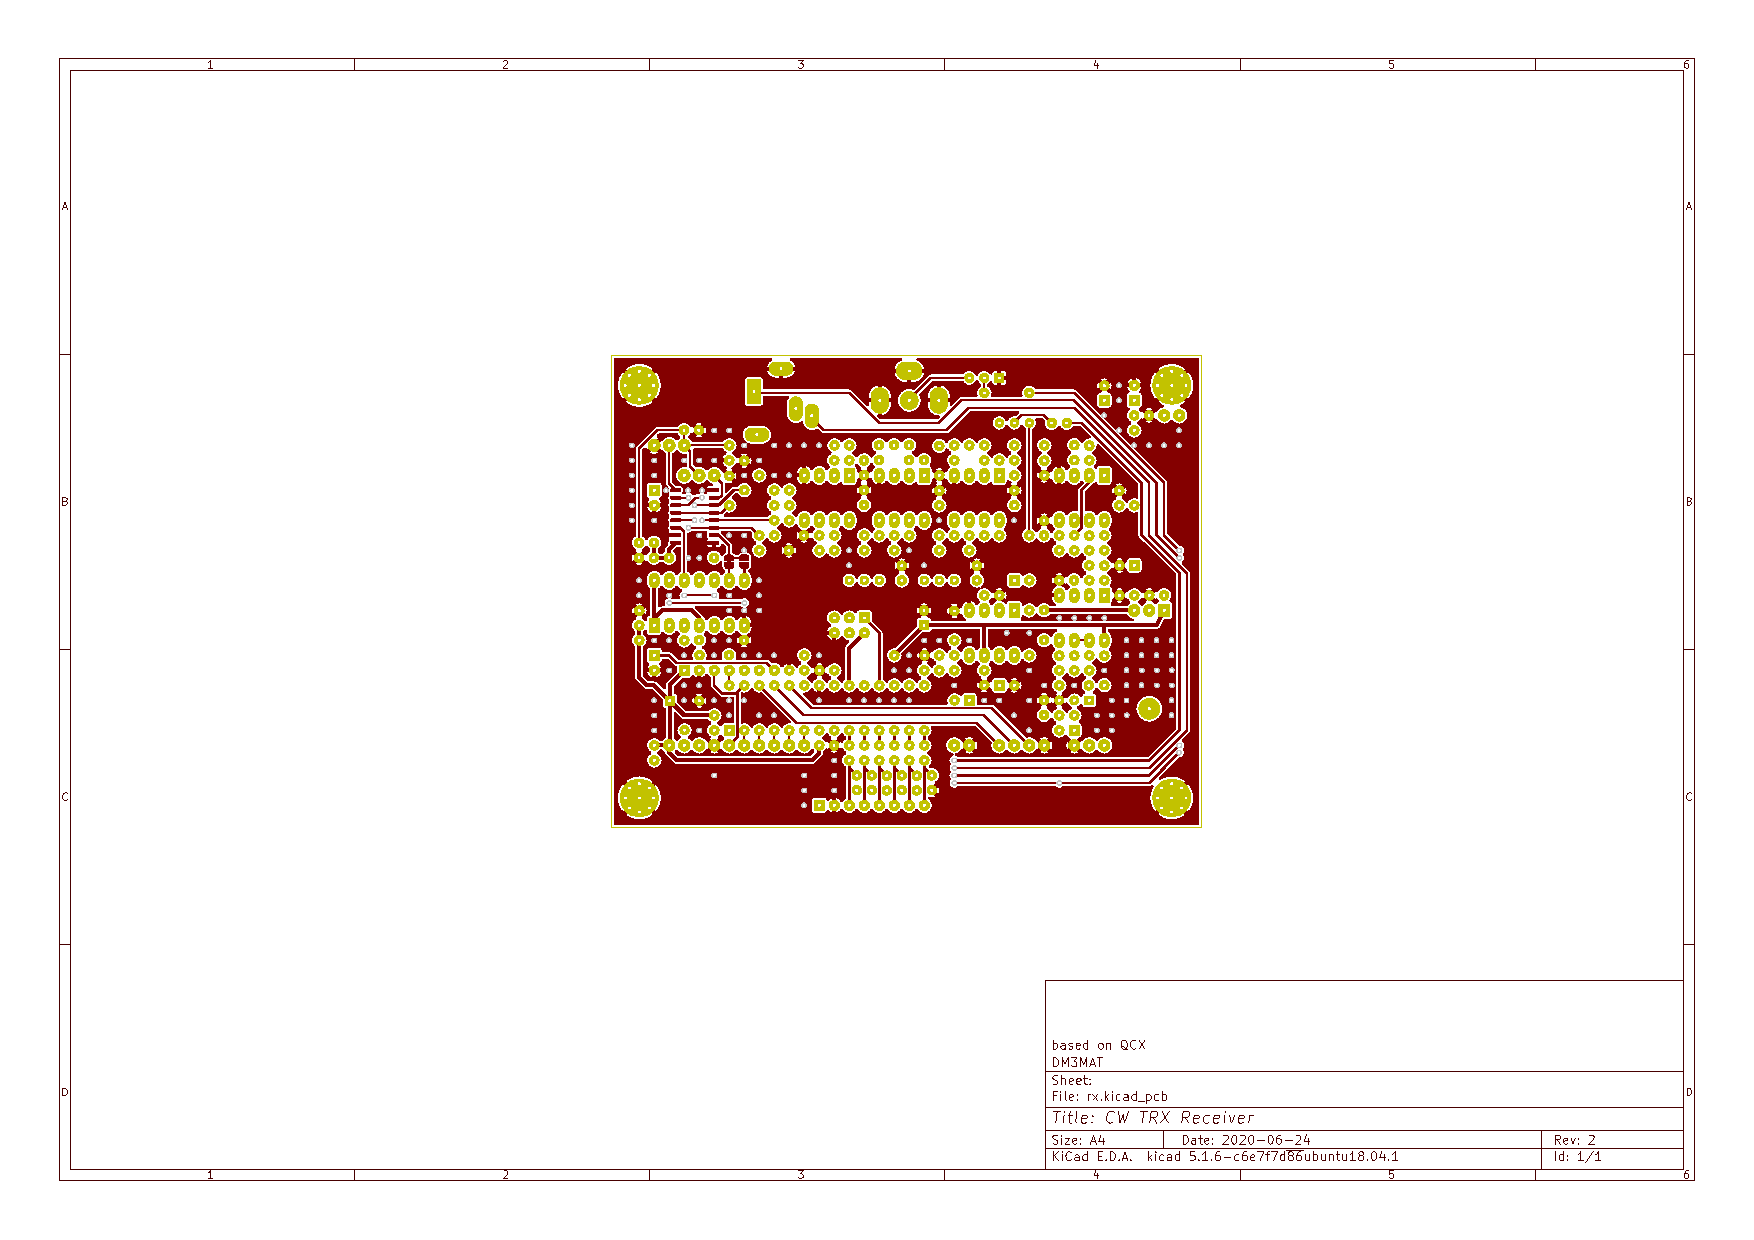
\includepdf[pages={1,2,3},landscape=true, addtotoc={
 1, section, 1, RX Board, rxbrdtop,
 2, subsection, 1, Bottom, rxbrdbottom,
 3, subsection, 1, Silkscreen, rxbrdsilk}]{fig/rx_brd.pdf}
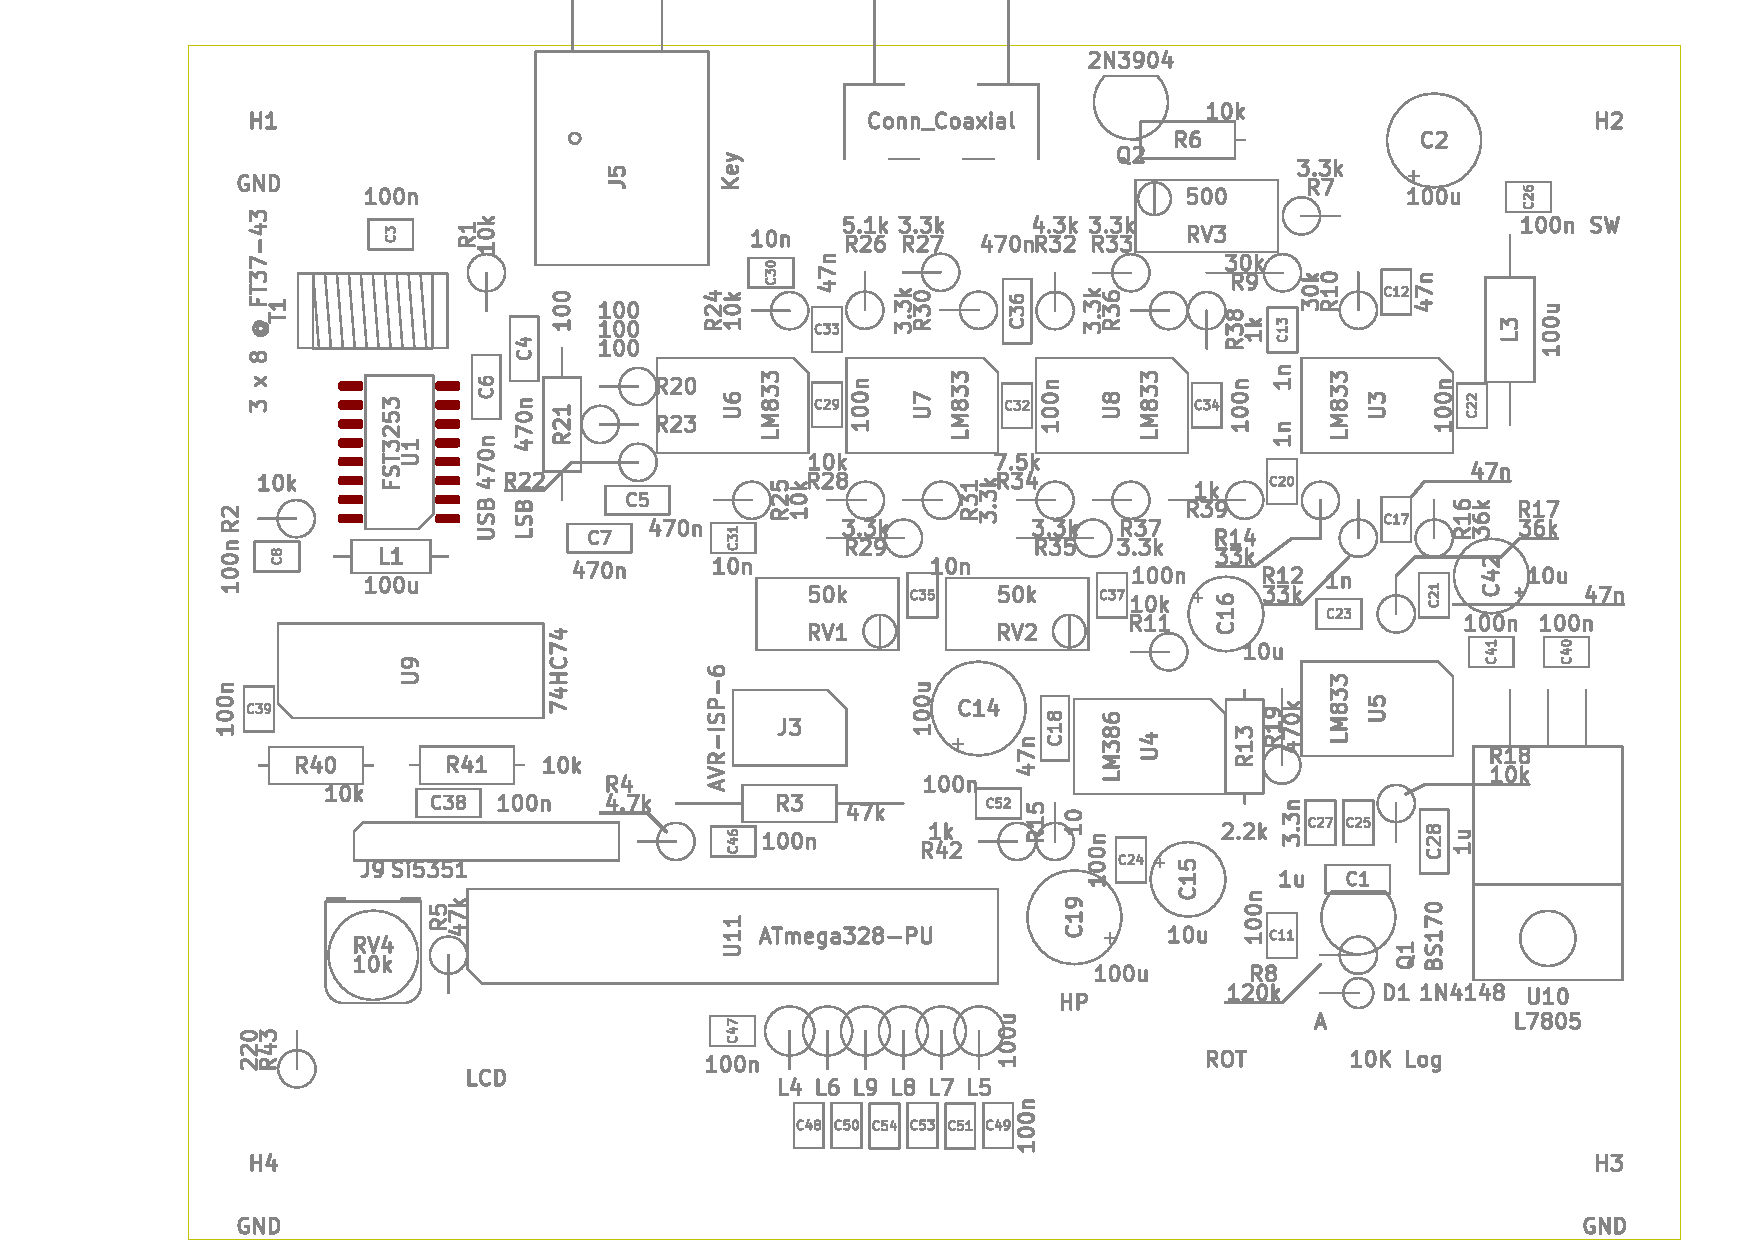
\includepdf[landscape=true, addtotoc={
 1, subsection, 1, Component Placement \& Values, rxval}]{fig/rx_values.pdf}
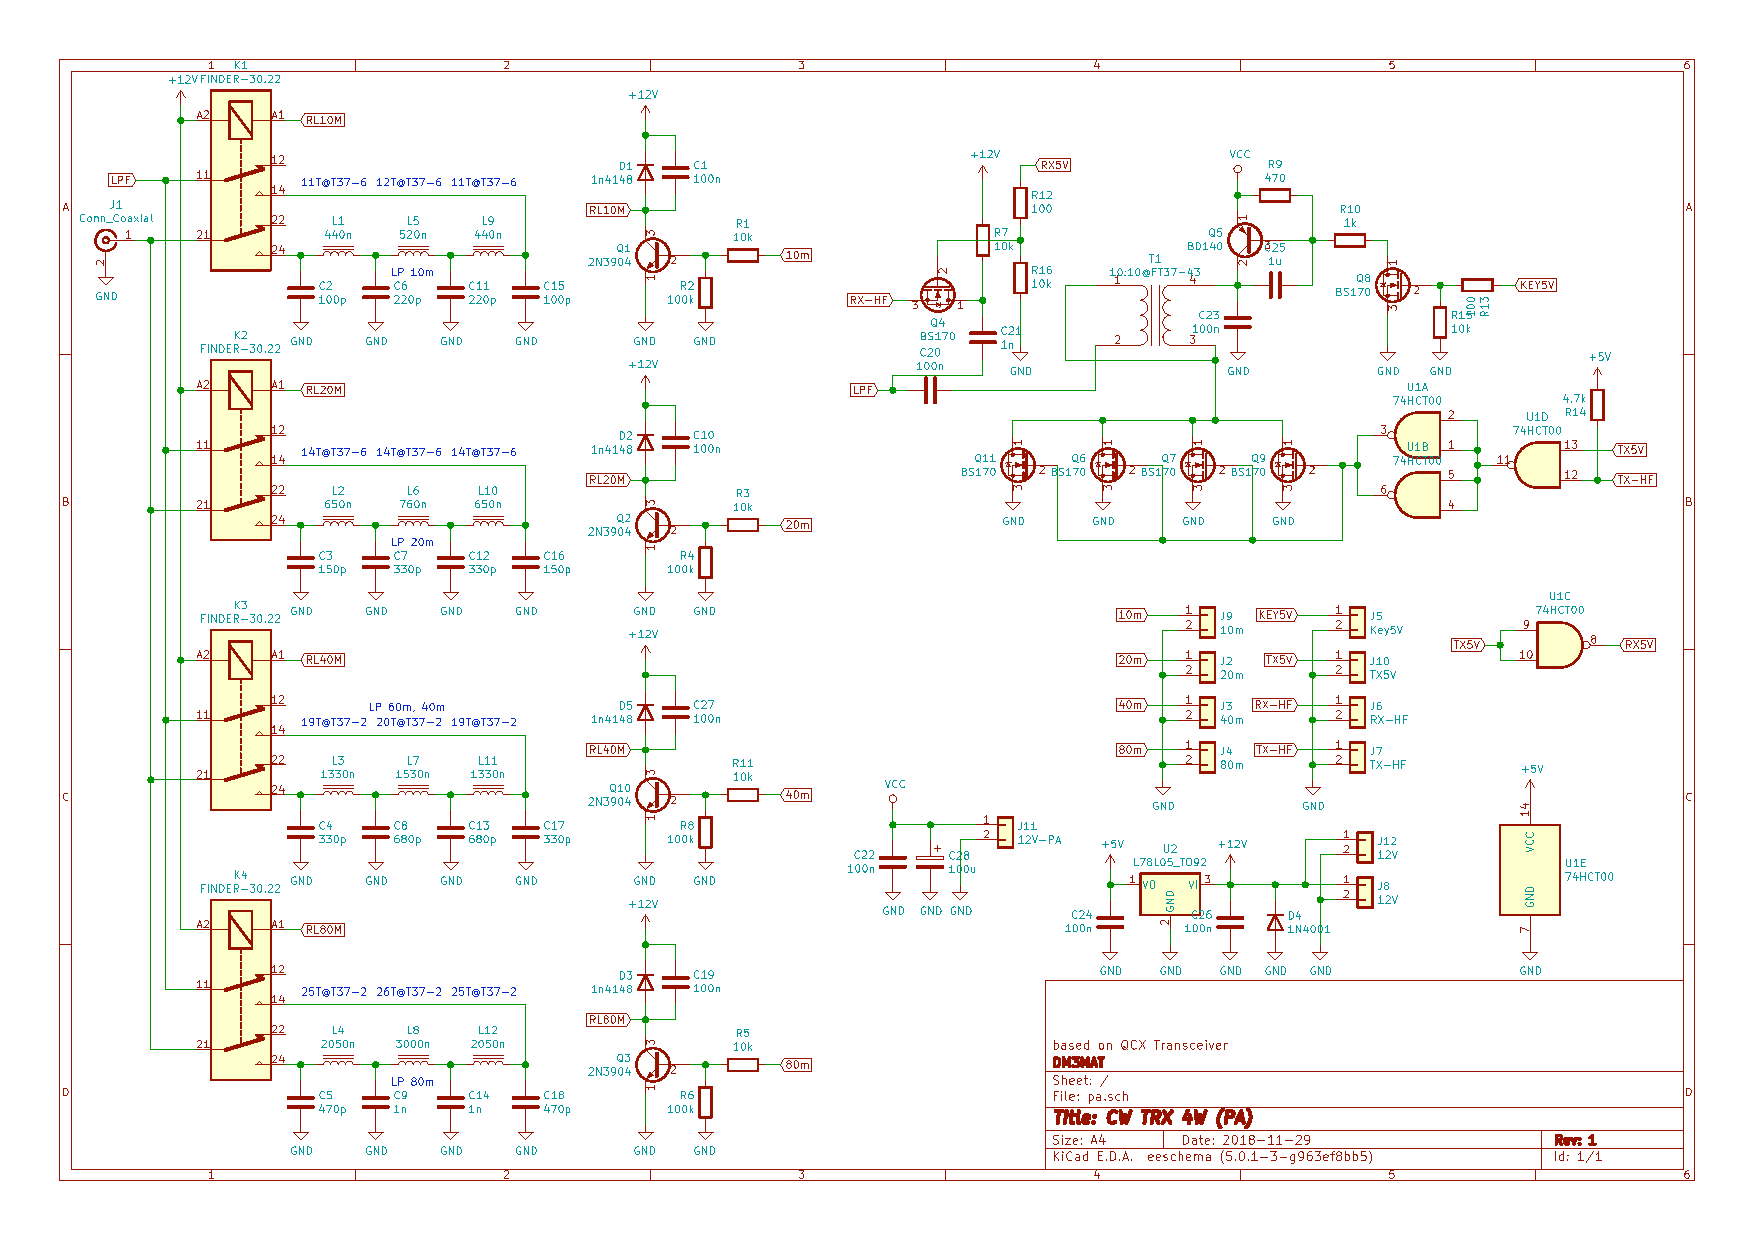
\includepdf[landscape=true, addtotoc={
 1, section, 1, PA/LP Circuit, pascm}]{fig/pa_scm.pdf}
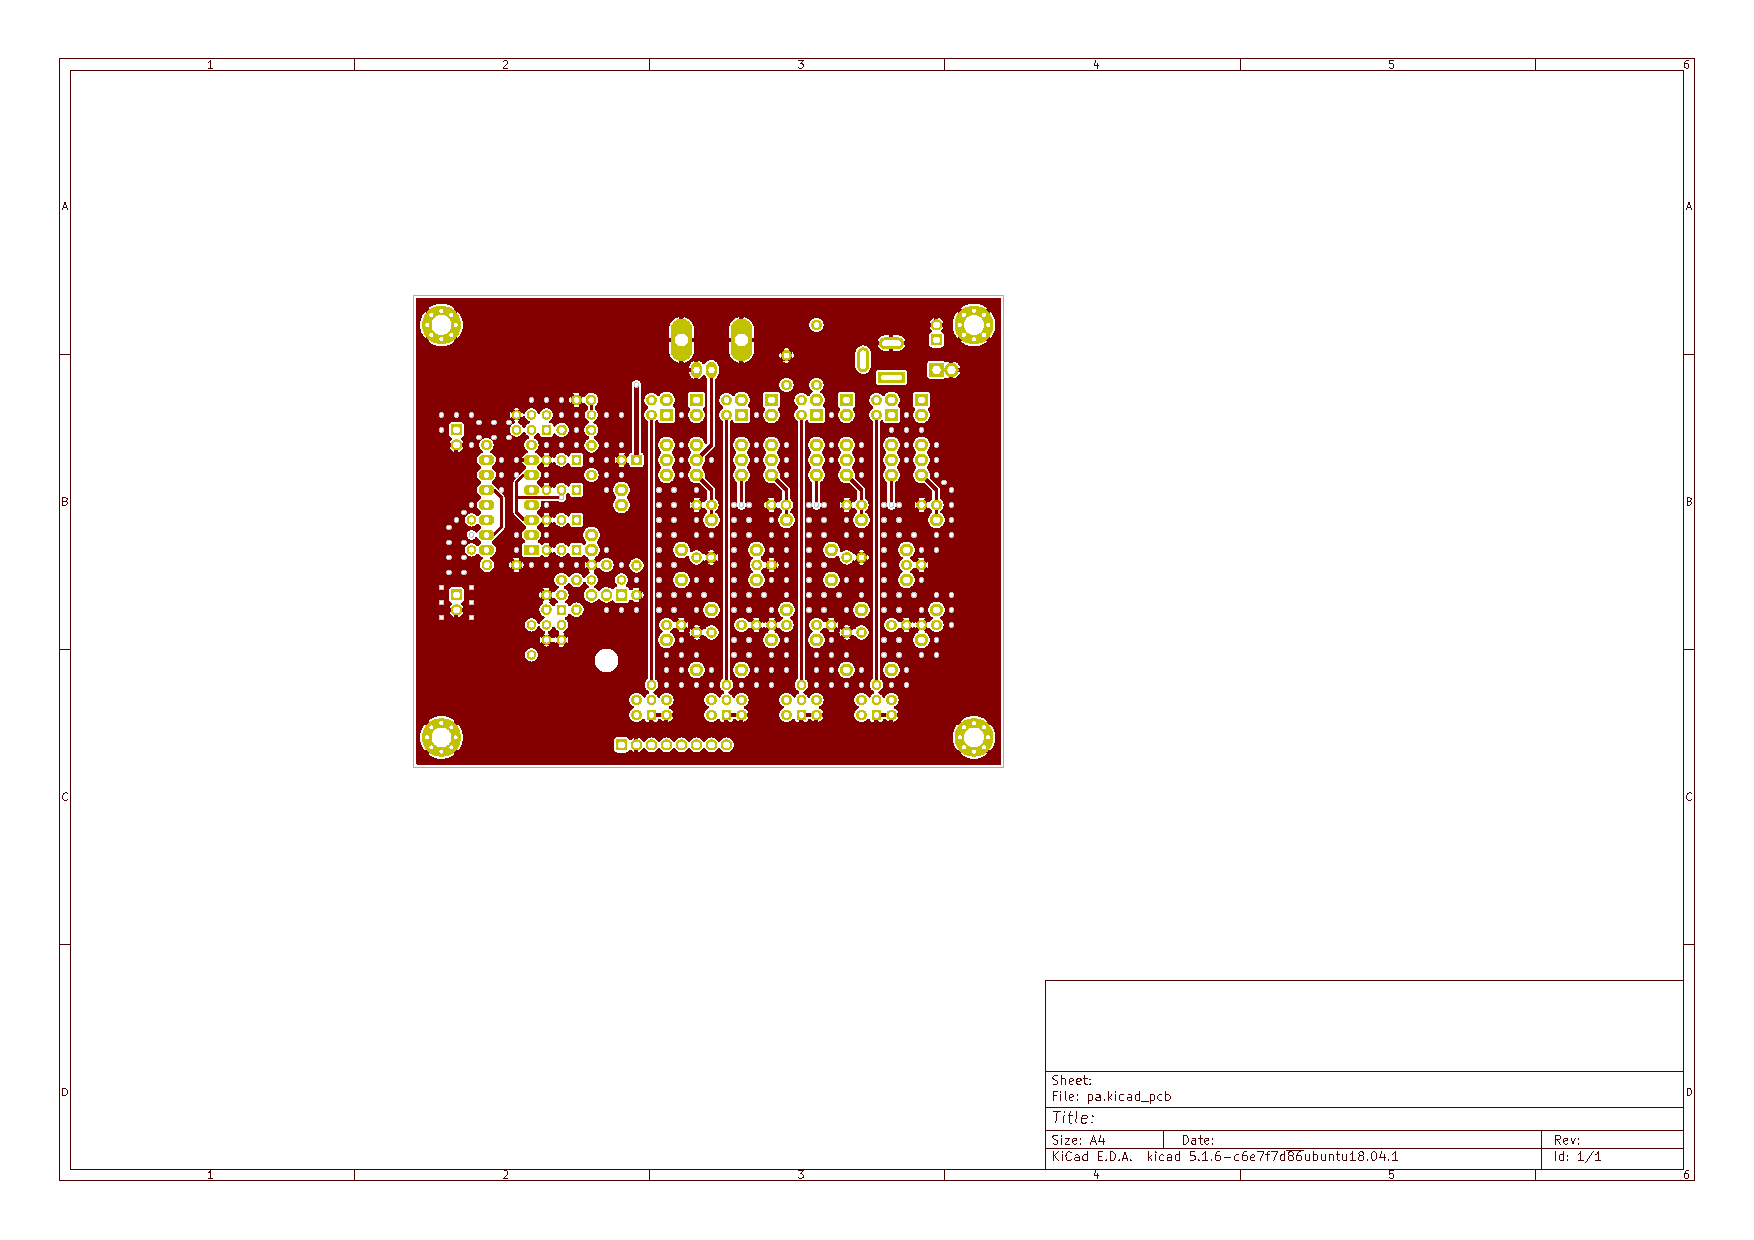
\includepdf[pages={1,2,3},landscape=true, addtotoc={
 1, section, 1, PA/LP Board, pabrdtop,
 2, subsection, 1, Bottom, pabrdbottom,
 3, subsection, 1, Silkscreen, pabrdsilk}]{fig/pa_brd.pdf}
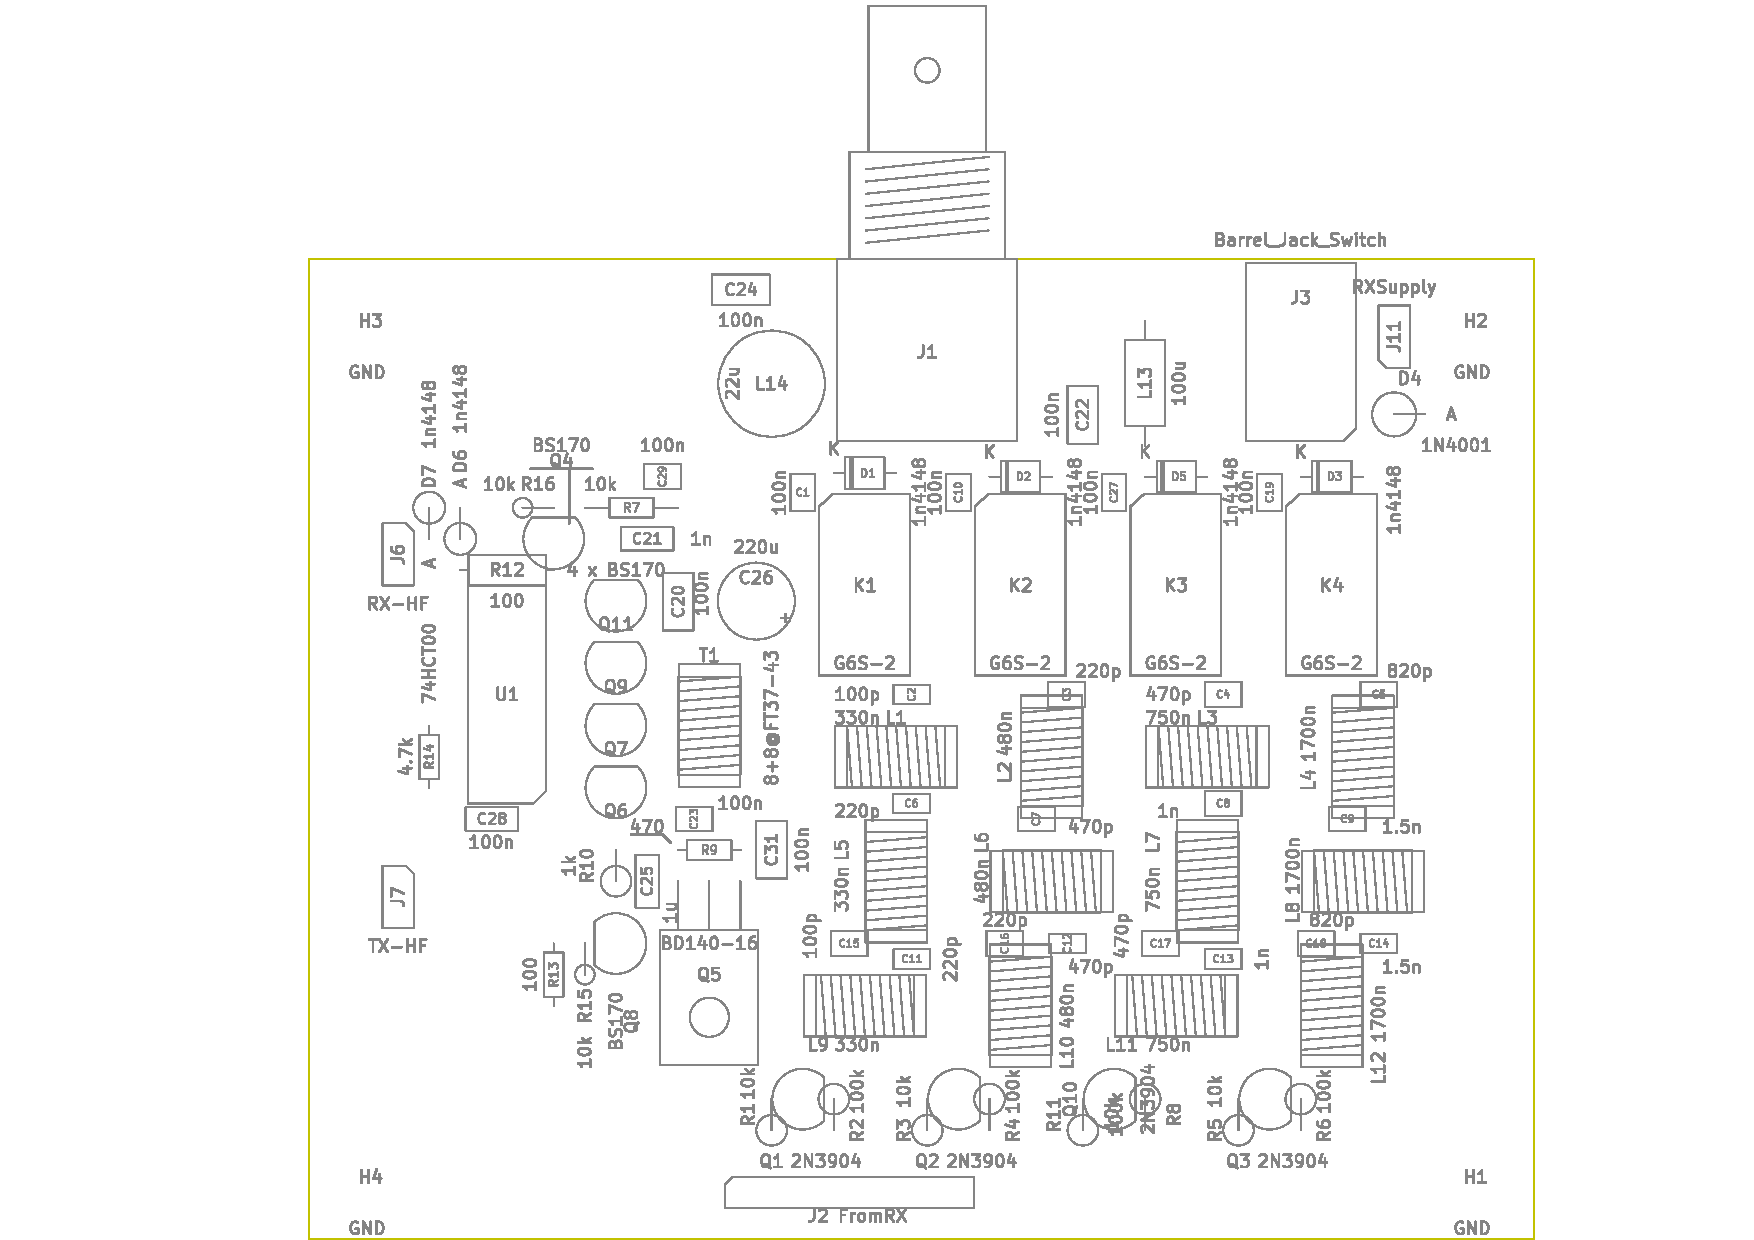
\includepdf[landscape=true, addtotoc={
 1, subsection, 1, Component Placement \& Values, pacomp}]{fig/pa_values.pdf}
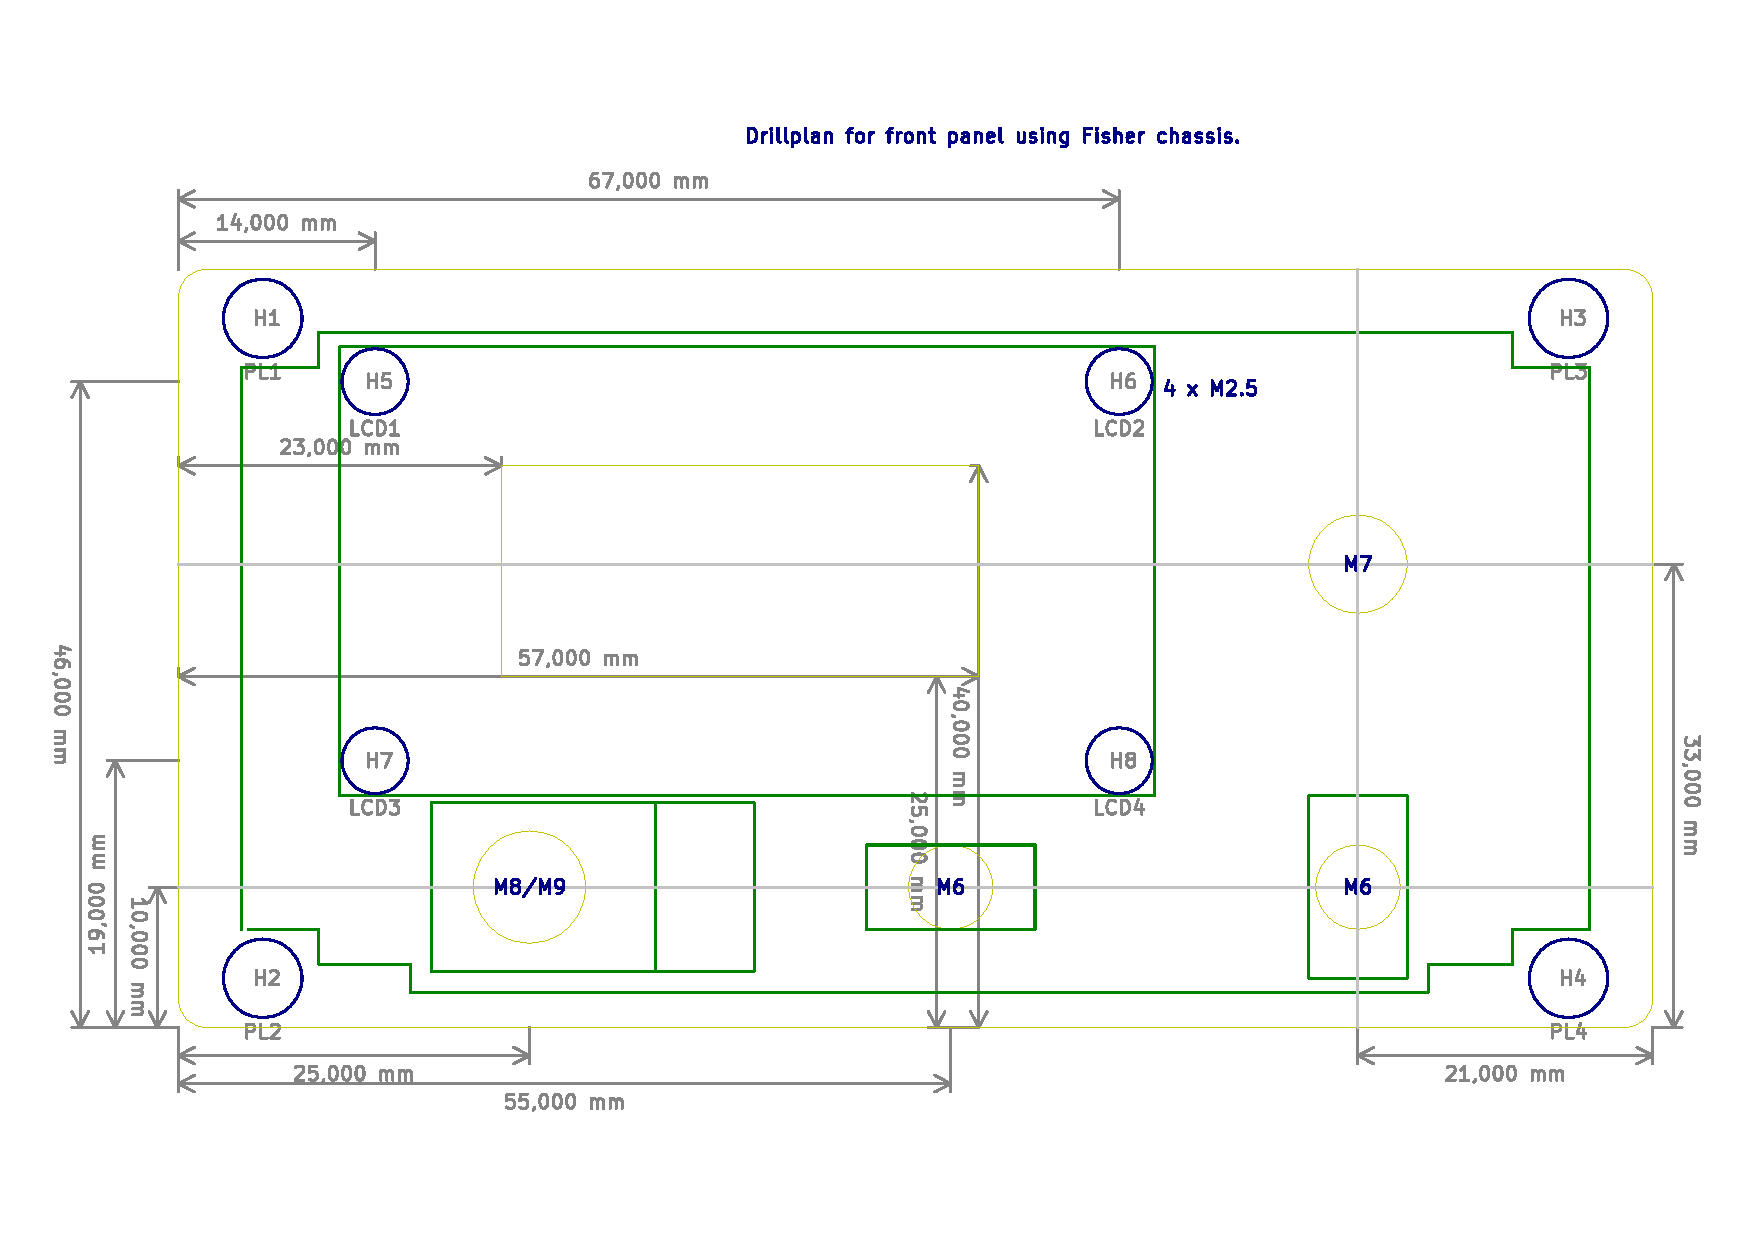
\includepdf[landscape=true, addtotoc={
 1, section, 1, Drill Plan, drillfront}]{fig/drill_front.pdf}
\end{document}